%% Chapter 2: a mathematical toolkit (new for the book)
% chapter macros
\DeclareRobustCommand{\PD}{\mathrm{PD}}
\DeclareRobustCommand{\GEM}{\mathrm{GEM}}
\DeclareRobustCommand{\Be}{\mathrm{Be}}
\DeclareRobustCommand{\Ga}{\mathrm{Ga}}
\DeclareRobustCommand{\Dir}{\mathrm{Dir}}
\DeclareRobustCommand{\PG}{\mathrm{PG}}
\DeclareRobustCommand{\DP}{\mathrm{DP}}
\DeclareRobustCommand{\Bin}{\mathrm{Bin}}
\DeclareRobustCommand{\Po}{\mathrm{Po}}
\DeclareRobustCommand{\one}{\mathbf{1}}
\chapter{A Mathematical Toolkit}\label{ch:toolkit}
\chaptermark{A Mathematical Toolkit}

\begin{chaptersummary}
The later chapters of this book draw on four bodies of mathematics that are rarely found between
the same covers: the classical theory of genotype frequencies and quantitative genetics, the
stochastic theory of drift in finite populations, the theory of exchangeable random partitions
that grew out of the Ewens sampling formula, and a set of Bayesian and likelihood free
computational devices. This chapter collects what is needed, in the notation used later, with
definitions, short proofs and at least one worked numerical example for each topic. We cover
Hardy Weinberg proportions and linkage disequilibrium; average effects as a weighted least
squares projection and the additive genetic variance; the Wright Fisher and Moran models, the
diffusion approximation and Kimura's fixation probability; exchangeability, de Finetti's
theorem, the P\'olya urn, the Dirichlet distribution and process, stick breaking and the two
parameter Poisson Dirichlet family; the Ewens and Pitman sampling formulae, the number of alleles
and Fisher's logarithmic series; the Kingman coalescent with Watterson's estimator and the site
frequency spectrum; global local shrinkage, the horseshoe and several data augmentation
identities; and rejection approximate Bayesian computation, the check loss and the noise
outsourcing lemma. Every number in the chapter has been checked by exact computation or
simulation.
\end{chaptersummary}

\section{How to use this chapter}\label{toolkit:sec:use}

This chapter is a reference, not an argument. Each of the later chapters is self contained and
introduces its own notation, but each also assumes some background that a statistician may lack
on the genetic side or a geneticist may lack on the probabilistic side. The sections below supply
that background in the order in which the book uses it.
Section~\ref{toolkit:sec:hw} is needed for Part I (Chapters~\ref{ch:ftns}, \ref{ch:hs} and
\ref{ch:mp}); Sections~\ref{toolkit:sec:exch} and \ref{toolkit:sec:esf} for Part II
(Chapters~\ref{ch:esf} to \ref{ch:rc}); Sections~\ref{toolkit:sec:drift} and
\ref{toolkit:sec:coal} for Part III (Chapters~\ref{ch:suff} and \ref{ch:coal}); and
Sections~\ref{toolkit:sec:bayes} and \ref{toolkit:sec:lfi} throughout.

A reader who knows a topic can skip its section; nothing later depends on the proofs here, only
on the statements. We have nevertheless given proofs, or sketches that a reader can complete,
because several of the identities (the projection formula for average effects, the spectrum
identity $\E\xi_i=\theta/i$, the Beta augmentation of a ratio of Gamma functions) are used later
in ways that only make sense once one has seen why they are true. Worked examples use small
numbers that can be checked by hand; the scripts that check them are in the directory
\texttt{code/toolkit} that accompanies the book.

Two conventions hold throughout. The rising factorial is
$(x)_m=x(x+1)\cdots(x+m-1)$, with $(x)_0=1$, so that $(x)_m=\Gamma(x+m)/\Gamma(x)$; the
book also writes it $x^{(m)}$. Population sizes are counted in genes: a population of $N$ genes
is a haploid population of $N$ individuals or a diploid population of $N_d=N/2$ individuals, and we
say so whenever the distinction matters. In this chapter, therefore, the scaled mutation rate is
$\theta=2N\mu$ and coalescent time is measured in units of $N$ generations. Most other
chapters (Chapters~\ref{ch:intro}, \ref{ch:ftns}, \ref{ch:mp}, \ref{ch:pig}, \ref{ch:rc},
\ref{ch:suff} and \ref{ch:coal}) instead write $N$ for the number of diploid individuals, or for the effective size
$N_e$, so that their $\theta=4N\mu$ and their time unit of $2N$ generations are the same
quantities as $\theta=2N\mu$ and $N$ generations here; the $\theta$ itself, and every formula
stated in terms of $\theta$, is unchanged.

%% ======================================================================
\section{Genotypes, gametes and the additive model}\label{toolkit:sec:hw}

This section sets out the static theory of a Mendelian population: how genotype frequencies
relate to gene frequencies, how two loci are associated, and how a genotypic value is split into
an additive part and a remainder. These are the objects of Fisher's Fundamental Theorem in
Part I, and the projection of Section~\ref{toolkit:sec:avg} is the lemma on which
Chapters~\ref{ch:ftns} to \ref{ch:mp} are built.

\subsection{Hardy Weinberg proportions}\label{toolkit:sec:hwlaw}

Consider an autosomal locus with alleles $A_1,\dots,A_k$ in a diploid population. Write
$P_{ij}$ for the frequency of the unordered genotype $A_iA_j$, so that $\sum_{i\le j}P_{ij}=1$,
and $p_i=P_{ii}+\tfrac12\sum_{j\ne i}P_{ij}$ for the frequency of $A_i$ among genes.

\begin{definition}[Hardy Weinberg proportions]\label{toolkit:def:hw}
A genotype distribution is in Hardy Weinberg proportions if $P_{ii}=p_i^2$ and
$P_{ij}=2p_ip_j$ for $i<j$; equivalently, if the two genes of a random individual are
independent draws from $(p_1,\dots,p_k)$.
\end{definition}

The intuition is that Mendelian segregation hands each offspring one gene drawn at random from
each parent, so if parents pair at random the offspring's two genes are independent draws from
the gene pool. Nothing in the argument depends on the parental genotype frequencies.

\begin{theorem}[Hardy and Weinberg]\label{toolkit:thm:hw}
Suppose generations are discrete, mating is at random, the gene frequencies are the same in the
two sexes, there is no selection, mutation or migration, and the population is infinite.
Then whatever the parental genotype frequencies, the offspring are in Hardy Weinberg proportions
with the parental gene frequencies $p_i$, and the population remains so in every later
generation.
\end{theorem}

\begin{proof}
A gamete from a random parent carries $A_i$ with probability $P_{ii}+\tfrac12\sum_{j\ne
i}P_{ij}=p_i$, by Mendel's first law. Under random mating the two gametes forming a zygote come
from independent parents, so the ordered pair of genes is $(A_i,A_j)$ with probability
$p_ip_j$, giving $P'_{ii}=p_i^2$ and $P'_{ij}=2p_ip_j$. The gene frequencies of the offspring
are $p_i^2+\tfrac12\sum_{j\ne i}2p_ip_j=p_i$, so the next generation is formed from the same
$p_i$ and the argument repeats.
\end{proof}

The theorem is a statement about geometry as much as about genetics. The genotype frequencies
live in a simplex of dimension $k(k+1)/2-1$; the Hardy Weinberg distributions form a smooth
submanifold of dimension $k-1$, parametrised by the gene frequencies, consisting of the
symmetric product measures $p\otimes p$. Random mating projects any point of the simplex onto
this manifold in one generation along the fibres of constant gene frequency. In
Chapter~\ref{ch:ftns} the Fundamental Theorem is shown to hold exactly when the population moves
tangentially to the corresponding manifold for many loci, and a transverse coordinate at one
biallelic locus can be taken to be the inbreeding coefficient $F$ (that chapter uses Lindley's log cross product ratio, a function of $F$ and $p$), defined by
\begin{equation}\label{toolkit:eq:F}
P_{11}=p^2+Fpq,\qquad P_{12}=2pq(1-F),\qquad P_{22}=q^2+Fpq,\qquad q=1-p.
\end{equation}
Every biallelic genotype distribution with $0<p<1$ can be written this way for a unique $F$,
which measures the excess of homozygotes; Hardy Weinberg is $F=0$.

\begin{example}[Ford's scarlet tiger moth]\label{toolkit:ex:moth}
Ford's sample of the scarlet tiger moth \emph{Panaxia dominula} from Cothill, a standard textbook
data set \citep{toolkit:ford1971}, contained $1469$ of the common homozygote, $138$
heterozygotes and $5$ of the rare homozygote, $n=1612$ in all. The common allele has frequency
$\hat p=(2\cdot1469+138)/3224=0.9541$. The Hardy Weinberg expectations are $n\hat p^2=1467.4$,
$2n\hat p\hat q=141.2$ and $n\hat q^2=3.4$, and Pearson's statistic is
$\sum(O-E)^2/E=0.83$ on one degree of freedom ($p$ value $0.36$). The estimated inbreeding
coefficient is $\hat F=1-(138/1612)/(2\hat p\hat q)=0.023$. The data sit on the Hardy Weinberg
manifold to within sampling error.
\end{example}

\subsection{Two loci and linkage disequilibrium}\label{toolkit:sec:ld}

With two biallelic loci, alleles $A,a$ and $B,b$, a gamete is one of four haplotypes $AB$,
$Ab$, $aB$, $ab$ with frequencies $x_{AB},x_{Ab},x_{aB},x_{ab}$. The marginal frequencies are
$p_A=x_{AB}+x_{Ab}$ and $p_B=x_{AB}+x_{aB}$.

\begin{definition}[Linkage disequilibrium]\label{toolkit:def:ld}
The coefficient of linkage disequilibrium is $D=x_{AB}-p_Ap_B$. The population is in linkage
equilibrium if $D=0$, that is, if the haplotype distribution is the product of its marginals.
\end{definition}

Expanding $x_{AB}(1-x_{AB}-x_{Ab}-x_{aB})-x_{Ab}x_{aB}=x_{AB}-(x_{AB}+x_{Ab})(x_{AB}+x_{aB})$
gives the symmetric form
\begin{equation}\label{toolkit:eq:Dcross}
D=x_{AB}\,x_{ab}-x_{Ab}\,x_{aB},
\end{equation}
the determinant of the $2\times2$ table of haplotype frequencies. The haplotype simplex has
dimension three, the product measures form a surface of dimension two, and $D$ is the
coordinate transverse to it. Two normalised versions are common: $r^2=D^2/(p_Aq_Ap_Bq_B)$, the
squared correlation between the allelic indicators, and $D'=D/D_{\max}$ with
$D_{\max}=\min(p_Aq_B,q_Ap_B)$ when $D>0$.

The next result says that recombination drives $D$ to zero geometrically without changing the
gene frequencies.

\begin{proposition}[Decay of disequilibrium]\label{toolkit:prop:ldecay}
Under random mating with recombination fraction $c$ between the loci, and no other forces,
$p_A$ and $p_B$ are constant and $D_{t+1}=(1-c)D_t$, so $D_t=(1-c)^tD_0$.
\end{proposition}

\begin{proof}
A gamete produced by an individual is a parental haplotype with probability $1-c$ and a
recombinant with probability $c$. A parental haplotype is $AB$ with probability $x_{AB}$. A
recombinant takes its $A$ locus allele from one of the parent's two haplotypes and its $B$ locus
allele from the other; under random mating these are independent draws from the haplotype pool,
so the recombinant is $AB$ with probability $p_Ap_B$. Hence $x'_{AB}=(1-c)x_{AB}+cp_Ap_B$, and
subtracting $p_Ap_B$ gives $D'=(1-c)D$. The marginals are unchanged because recombination only
reshuffles alleles between loci.
\end{proof}

\begin{example}[Disequilibrium and its decay]\label{toolkit:ex:ld}
Take $x_{AB}=0.5$, $x_{Ab}=x_{aB}=0.1$, $x_{ab}=0.3$. Then $p_A=p_B=0.6$, $D=0.5-0.36=0.14$, and
\eqref{toolkit:eq:Dcross} gives the same value $0.15-0.01$. The correlation is
$r^2=0.14^2/0.24^2=0.340$ and $D'=0.14/0.24=0.583$. With $c=0.1$ the disequilibrium after $1$,
$5$, $10$ and $20$ generations is $0.126$, $0.083$, $0.049$ and $0.017$; iterating the haplotype
recursion directly reproduces these values. Loosely linked loci forget their association quickly;
tightly linked loci, with $c$ near zero, preserve it for many generations, which is why
disequilibrium maps the genome.
\end{example}

\subsection{Average effects as a projection}\label{toolkit:sec:avg}

Fisher's average effect is the central quantity of Part I, and it is defined most cleanly as a
regression coefficient \citep{toolkit:fisher1918,toolkit:fisher1941}. Take one biallelic locus,
alleles $A_1$ and $A_2$ with frequencies $p$ and $q=1-p$, genotype frequencies $P_g$ for
$g\in\{11,12,22\}$, and genotypic values $G_{11},G_{12},G_{22}$ (the mean phenotype, or the
fitness, of each genotype). Let $X_g\in\{2,1,0\}$ count the copies of $A_1$ and
$\mu=\sum_gP_gG_g$. Work in the space of functions on the three genotypes with the inner product
$\langle f,h\rangle_P=\sum_gP_gf_gh_g$.

\begin{definition}[Average excess, average effect, breeding value]\label{toolkit:def:avg}
The average excess of $A_1$ is the mean genotypic value of the carriers of a randomly chosen
$A_1$ gene, less $\mu$:
\[
e_1=\frac{P_{11}G_{11}+\tfrac12P_{12}G_{12}}{p}-\mu,\qquad
e_2=\frac{P_{22}G_{22}+\tfrac12P_{12}G_{12}}{q}-\mu .
\]
The average effect $\alpha$ of substituting $A_1$ for $A_2$ is the slope of the weighted least
squares regression of $G$ on $X$ with weights $P$:
\[
(\mu_0,\alpha)=\arg\min_{(m,b)}\;\sum_gP_g\,(G_g-m-bX_g)^2 .
\]
The breeding value is the fitted value centred at the mean, $A_g=\alpha(X_g-2p)$, and the
dominance deviation is the residual $\delta_g=G_g-\mu-A_g$.
\end{definition}

So the breeding value is the orthogonal projection of $G-\mu$ onto the span of $X-2p$ in the
inner product $\langle\cdot,\cdot\rangle_P$, and the dominance deviation is orthogonal to both
constants and $X$. The point that Chapter~\ref{ch:ftns} turns on is already visible: the
subspace (functions linear in gene content) is fixed, but the inner product moves with the
genotype frequencies.

\begin{theorem}[Average effect and average excess]\label{toolkit:thm:avg}
For any genotype frequencies of the form \eqref{toolkit:eq:F},
\begin{equation}\label{toolkit:eq:alphaF}
pe_1+qe_2=0,\qquad \alpha=\frac{e_1-e_2}{1+F}.
\end{equation}
Under Hardy Weinberg proportions, $\alpha=e_1-e_2=a+d(q-p)$, where $a=(G_{11}-G_{22})/2$ and
$d=G_{12}-(G_{11}+G_{22})/2$, and the variance of $G$ splits orthogonally as
\begin{equation}\label{toolkit:eq:vardecomp}
\sigma^2_G=\sigma^2_A+\sigma^2_D,\qquad \sigma^2_A=2pq\,\alpha^2,\qquad \sigma^2_D=(2pqd)^2 .
\end{equation}
\end{theorem}

\begin{proof}
First, $pe_1+qe_2=P_{11}G_{11}+P_{12}G_{12}+P_{22}G_{22}-(p+q)\mu=0$. The weighted least squares
slope is $\Cov_P(X,G)/\Var_P(X)$. Since $p=P_{11}+\tfrac12P_{12}$,
\[
\Cov_P(X,G)=\sum_gP_gX_g(G_g-\mu)=2P_{11}(G_{11}-\mu)+P_{12}(G_{12}-\mu)=2pe_1 .
\]
From $pe_1=-qe_2$ we get $e_1-e_2=e_1(1+p/q)=e_1/q$, so $\Cov_P(X,G)=2pq(e_1-e_2)$. Under
\eqref{toolkit:eq:F}, $\E_PX^2=4(p^2+Fpq)+2pq(1-F)$ and $\E_PX=2p$, so
$\Var_P(X)=2pq(1+F)$, which proves \eqref{toolkit:eq:alphaF}. At $F=0$,
$e_1=pG_{11}+qG_{12}-\mu$ and $e_2=pG_{12}+qG_{22}-\mu$; writing $G_{11}=m+a$, $G_{12}=m+d$,
$G_{22}=m-a$ gives $e_1-e_2=p(a-d)+q(d+a)=a+d(q-p)$. The decomposition
\eqref{toolkit:eq:vardecomp} is Pythagoras in $\langle\cdot,\cdot\rangle_P$, since $\delta$ is
orthogonal to $A$; $\sigma^2_A=\alpha^2\Var_P(X)=2pq\alpha^2$. Finally a direct computation gives
$\delta_{11}=-2q^2d$, $\delta_{12}=2pqd$, $\delta_{22}=-2p^2d$, whence
$\sigma^2_D=4p^2q^2d^2(q^2+2pq+p^2)=(2pqd)^2$.
\end{proof}

The theorem says that average excess and average effect coincide exactly when the population is
in Hardy Weinberg proportions, and differ by the factor $1+F$ otherwise. Fisher's 1941 paper drew
this distinction; Chapter~\ref{ch:ftns} shows that the gap between the two is the one dimensional
shadow of the term Fisher's theorem neglects.

\begin{example}[One locus with partial dominance]\label{toolkit:ex:avg}
Let $p=0.4$ and $(G_{11},G_{12},G_{22})=(10,8,4)$, so $a=3$ and $d=1$. Under Hardy Weinberg the
genotype frequencies are $(0.16,0.48,0.36)$ and $\mu=6.88$. The average excesses are
$e_1=0.4\cdot10+0.6\cdot8-6.88=1.92$ and $e_2=0.4\cdot8+0.6\cdot4-6.88=-1.28$, and indeed
$0.4\cdot1.92-0.6\cdot1.28=0$. The average effect is $\alpha=3.2=a+d(q-p)=3+0.2$, and the
weighted regression of $G$ on $X$ returns intercept $4.32$ and slope $3.2$. The breeding values
are $(3.84,0.64,-2.56)$ and the dominance deviations $(-0.72,0.48,-0.32)$. The variances are
\[
\sigma^2_G=5.1456,\qquad \sigma^2_A=2(0.24)(3.2)^2=4.9152,\qquad \sigma^2_D=(0.48)^2=0.2304,
\]
and they add. The proportion of genotypic variance that is additive is $0.955$: with only mild
dominance, almost all of the variance is transmissible. If instead the population carries excess
homozygosity $F=0.2$ at the same $p$, the genotype frequencies become $(0.208,0.384,0.408)$, the
weighted regression slope falls to $\alpha=3.133$, while $e_1-e_2=3.76=1.2\,\alpha$, exactly as
\eqref{toolkit:eq:alphaF} predicts.
\end{example}

With many loci the same construction applies with $X$ replaced by the vector of gene contents at
all loci, and $\sigma^2_A$ is then the variance of the projection onto the span of those
contents. When the loci are in Hardy Weinberg and linkage equilibrium the gene contents at
different loci are uncorrelated, the projection splits locus by locus, and $\sigma^2_A$ is the
sum of the single locus values. Otherwise the regression must be fitted jointly, and with more
loci than individuals it is the overparametrised regression of Chapters~\ref{ch:hs}
and~\ref{ch:mp}.

%% ======================================================================
\section{Drift: the Wright Fisher and Moran models}\label{toolkit:sec:drift}

This section introduces the two standard models of a finite population, shows how their gene
frequency fluctuates, and derives the probability that a new allele is fixed. These results are
the forward time counterpart of the coalescent of Section~\ref{toolkit:sec:coal}, and they supply
the scaled parameters such as $\theta$ that appear in every later chapter. The standard reference for this
material, and for much of Sections~\ref{toolkit:sec:esf} and \ref{toolkit:sec:coal}, is
\citet{toolkit:ewens2004}.

\subsection{The two models}\label{toolkit:sec:wfmoran}

\begin{definition}[Wright Fisher model]\label{toolkit:def:wf}
A population of $N$ genes, $i$ of type $A$, produces the next generation by $N$ independent draws
from a gamete pool in which $A$ has frequency $\psi(i/N)$. Thus
$X_{t+1}\mid X_t=i\sim\Bin(N,\psi(i/N))$. Without selection $\psi(x)=x$; with genic selection of
strength $s$ in favour of $A$, $\psi(x)=x(1+s)/(1+sx)$.
\end{definition}

\begin{definition}[Moran model]\label{toolkit:def:moran}
A population of $N$ genes changes by one event at a time. At each event an individual is chosen
to reproduce, with probability proportional to fitness ($1+s$ for $A$, $1$ for $a$), and an
individual chosen uniformly at random dies and is replaced by the offspring. There are $N$
events per generation.
\end{definition}

The Wright Fisher model has nonoverlapping generations and is the natural discrete model; the
Moran model has overlapping generations and is a birth and death chain, which makes many of its
quantities exactly computable. For a diploid population of $N_d$ individuals one takes
$N=2N_d$ genes.

\begin{proposition}[Neutral drift]\label{toolkit:prop:drift}
In the neutral Wright Fisher model the frequency $x_t=X_t/N$ is a martingale, the probability that
$A$ is eventually fixed is $x_0$, and the expected heterozygosity $H_t=\E[2x_t(1-x_t)]$ satisfies
$H_t=(1-1/N)^tH_0$.
\end{proposition}

\begin{proof}
$\E[x_{t+1}\mid x_t]=x_t$ by the binomial mean. The chain is absorbed at $0$ or $1$ in finite time
almost surely, and bounded martingales converge, so optional stopping gives
$x_0=\E x_\infty=\Prob(\text{fixation})$. For the heterozygosity,
$\E[x_{t+1}^2\mid x_t]=x_t^2+x_t(1-x_t)/N$, so $\E[x_{t+1}(1-x_{t+1})\mid
x_t]=x_t(1-x_t)(1-1/N)$; take expectations.
\end{proof}

Heterozygosity is lost at rate $1/N$ per generation, so drift acts on a time scale of $N$
generations. This is the reason population genetic results are stated in units of $N$ (or $2N_d$)
generations and in scaled parameters such as $Ns$ and $N\mu$.

\begin{example}[Heterozygosity in a population of twenty genes]\label{toolkit:ex:het}
With $N=20$ and $x_0=1/2$, $H_0=0.5$ and the proposition predicts $H_1=0.475$,
$H_5=0.3869$ and $H_{10}=0.2994$. Propagating the exact $21\times21$ transition matrix gives the
same three numbers to five decimals. After ten generations, a population of twenty genes has
lost forty percent of its variation to chance alone.
\end{example}

\subsection{The diffusion approximation}\label{toolkit:sec:diffusion}

In one Wright Fisher generation with weak selection the change $\Delta x=x_{t+1}-x_t$ has
\begin{align*}
\E[\Delta x\mid x]&=\psi(x)-x=sx(1-x)+O(s^2),\\
\Var[\Delta x\mid x]&=\frac{\psi(x)\{1-\psi(x)\}}{N}=\frac{x(1-x)}{N}+O\Big(\frac sN\Big).
\end{align*}
Both moments are of order $1/N$ when $s=O(1/N)$, and higher moments are of smaller order. As
$N\to\infty$ with $Ns$ fixed, the process $x_{\lfloor Nt\rfloor}$ converges to the diffusion on
$[0,1]$ with generator
\begin{equation}\label{toolkit:eq:generator}
\mathcal{L}f(x)=\tfrac12x(1-x)f''(x)+\sigma x(1-x)f'(x),\qquad \sigma=Ns,
\end{equation}
time being measured in units of $N$ generations. This is the approximation Fisher introduced in
1922 and Kimura made the main computational tool of the subject \citep{toolkit:kimura1962}. For
the Moran model the variance per generation is $2x(1-x)/N$ because each of the $N$ events changes
the count by exactly one with probability $2x(1-x)$ and otherwise leaves it unchanged; the same diffusion arises with $N$
replaced by $N/2$. The Moran model drifts twice as fast.

Quantities defined by absorption satisfy ordinary differential equations in the starting point.
If $u(x)$ is the probability of fixation from frequency $x$ and $T(x)$ the expected time to
absorption, then
\begin{equation}\label{toolkit:eq:backward}
\mathcal{L}u=0,\quad u(0)=0,\ u(1)=1;\qquad \mathcal{L}T=-1,\quad T(0)=T(1)=0 .
\end{equation}
These are obtained by conditioning on the first small step of the process, exactly as for a
random walk.

\subsection{Fixation probabilities}\label{toolkit:sec:fixation}

The intuition behind the next theorem is that selection pushes the frequency up at a rate
proportional to $Ns$, while drift spreads it at a rate independent of $s$; the fixation
probability balances the two, and depends on $s$ and $N$ only through their product.

\begin{theorem}[Kimura's formula]\label{toolkit:thm:kimura}
For the diffusion \eqref{toolkit:eq:generator}, the probability of fixation from frequency $x$ is
\begin{equation}\label{toolkit:eq:kimura}
u(x)=\frac{1-e^{-2Nsx}}{1-e^{-2Ns}} .
\end{equation}
For a new mutant, $x=1/N$, and $Ns\gg1$ with $s$ small, $u\approx1-e^{-2s}\approx2s$.
\end{theorem}

\begin{proof}
The equation $\tfrac12x(1-x)u''+Nsx(1-x)u'=0$ reduces on $(0,1)$ to $u''=-2Nsu'$, so
$u'(x)=Ce^{-2Nsx}$ and $u(x)=C'(1-e^{-2Nsx})$. The boundary condition $u(1)=1$ fixes $C'$. For
$x=1/N$ the numerator is $1-e^{-2s}$ and the denominator tends to one when $Ns$ is large.
\end{proof}

For a diploid population of $N_d$ individuals in which each copy of the favoured allele adds $s$
to fitness, $N=2N_d$ and \eqref{toolkit:eq:kimura} becomes the familiar
$u(x)=(1-e^{-4N_dsx})/(1-e^{-4N_ds})$, while a new mutant at $x=1/(2N_d)$ is fixed with
probability close to Haldane's $2s$. Even a strongly favoured mutant is usually lost: with
$s=0.01$ it survives with probability about two percent.

For the Moran model there is an exact answer. The number $i$ of $A$ genes moves up by one at rate
proportional to $(1+s)i(N-i)$ and down by one at rate proportional to $i(N-i)$, so it is a
gambler's ruin chain with ratio of down to up probabilities $r^{-1}$, $r=1+s$, and
\begin{equation}\label{toolkit:eq:moranfix}
u^{\mathrm{Moran}}_i=\frac{1-r^{-i}}{1-r^{-N}} .
\end{equation}

\begin{example}[Exact against diffusion for small populations]\label{toolkit:ex:kimura}
Table~\ref{toolkit:tab:fix} compares the exact fixation probability of a single new mutant in the
Wright Fisher model, obtained by solving the linear system for absorption probabilities of the
$(N+1)$ state chain, with Kimura's formula at $x=1/N$, and lists the exact Moran value
\eqref{toolkit:eq:moranfix}. Kimura's formula is accurate to within one percent when $Ns<1$
and to within three and a half percent when $s=0.1$, even for ten genes. The Moran values are
smaller, close to $s$ rather than $2s$ for large $Ns$, because the Moran model drifts twice as
fast; Kimura's formula with $N$ replaced by $N/2$ matches them to within five percent in every
case of the table. The exact neutral Wright Fisher answer is $1/N$, as
Proposition~\ref{toolkit:prop:drift} requires. For the mean absorption time from $x=1/2$, the
solution of $\mathcal{L}T=-1$ is $T(x)=-2\{x\log x+(1-x)\log(1-x)\}$ in units of $N$ generations,
so $T(1/2)=2N\log2=1.386N$ generations; the exact Wright Fisher values for $N=10$, $20$ and $50$ are $12.6$, $26.2$
and $67.5$ generations against $13.9$, $27.7$ and $69.3$ from the diffusion.
\end{example}

\begin{table}[t]
\centering\small
\caption{Fixation probability of a single new mutant in a population of $N$ genes.}
\label{toolkit:tab:fix}
\begin{tabular}{rrcccc}
\toprule
$N$ & $s$ & exact Wright Fisher & Kimura \eqref{toolkit:eq:kimura} & relative error & exact Moran\\
\midrule
10 & 0.01 & 0.1092 & 0.1092 & 0.0\% & 0.1045\\
10 & 0.05 & 0.1494 & 0.1505 & 0.8\% & 0.1233\\
10 & 0.10 & 0.2046 & 0.2096 & 2.5\% & 0.1480\\
20 & 0.01 & 0.0600 & 0.0601 & 0.1\% & 0.0549\\
20 & 0.05 & 0.1086 & 0.1101 & 1.3\% & 0.0764\\
20 & 0.10 & 0.1787 & 0.1847 & 3.3\% & 0.1068\\
50 & 0.01 & 0.0313 & 0.0313 & 0.2\% & 0.0253\\
50 & 0.05 & 0.0941 & 0.0958 & 1.8\% & 0.0522\\
50 & 0.10 & 0.1756 & 0.1813 & 3.3\% & 0.0917\\
\bottomrule
\end{tabular}
\end{table}

%% ======================================================================
\section{Exchangeability and random discrete distributions}\label{toolkit:sec:exch}

Part II of the book rests on one idea: a sample of genes whose order carries no information is
exchangeable, and an exchangeable sample behaves as if drawn independently from an unknown
random distribution. This section states that idea precisely and builds, step by step, the random
distributions that the Ewens and Pitman formulae sample from.

\subsection{De Finetti's theorem}\label{toolkit:sec:definetti}

\begin{definition}[Exchangeability]\label{toolkit:def:exch}
A sequence $X_1,X_2,\dots$ of random variables is exchangeable if for every $n$ and every
permutation $\pi$ of $\{1,\dots,n\}$, $(X_{\pi(1)},\dots,X_{\pi(n)})$ has the same law as
$(X_1,\dots,X_n)$.
\end{definition}

Independent identically distributed sequences are exchangeable, and so are mixtures of them. De
Finetti's theorem says that there is nothing else.

\begin{theorem}[de Finetti; Hewitt and Savage]\label{toolkit:thm:definetti}
Let $X_1,X_2,\dots$ be an exchangeable sequence taking values in a Polish space $\mathcal{X}$.
Then there is a unique probability measure $\Pi$ on the space of probability measures on
$\mathcal{X}$ such that for all $n$ and measurable $A_1,\dots,A_n$,
\[
\Prob(X_1\in A_1,\dots,X_n\in A_n)=\int\prod_{i=1}^nP(A_i)\,\Pi(\dd P).
\]
Moreover the empirical distribution $F_n=n^{-1}\sum_{i\le n}\delta_{X_i}$ converges weakly almost
surely to a random measure $P$ with law $\Pi$, and given $P$ the $X_i$ are independent with law
$P$.
\end{theorem}

\begin{proof}[Sketch for binary sequences]
Let $S_n=X_1+\dots+X_n$. Given $S_n=m$, exchangeability makes every arrangement of the $m$ ones
equally likely, so $X_1,\dots,X_k$ are the first $k$ draws without replacement from an urn with
$m$ ones and $n-m$ zeros. Hence for a fixed pattern with $r$ ones among the first $k$,
\[
\Prob(\text{pattern})=\sum_m\Prob(S_n=m)\frac{(m)_{r\downarrow}(n-m)_{(k-r)\downarrow}}{(n)_{k\downarrow}},
\]
where $(x)_{j\downarrow}=x(x-1)\cdots(x-j+1)$. Drawing with and without replacement differ by at
most $k(k-1)/(2n)$ in total variation, so the right side is
$\int p^r(1-p)^{k-r}\,\dd\Pi_n(p)+O(k^2/n)$ with $\Pi_n$ the law of $S_n/n$. By Helly's selection
theorem some subsequence $\Pi_{n_j}$ converges weakly to a measure $\Pi$ on $[0,1]$, and the
continuous integrand passes to the limit. Uniqueness follows because a measure on $[0,1]$ is
determined by its moments.
\end{proof}

The proof is the elementary one of \citet{toolkit:heath1976}; Chapter~\ref{ch:esf} gives it in
full for a general space, and \citet{toolkit:aldous1985} surveys the subject. The bound
$k(k-1)/(2n)$ is also the content of the finite form of the theorem
\citep{toolkit:diaconis1980}: the first $k$ of $n$ exchangeable variables are within $k(k-1)/(2n)$
in total variation of a mixture of independent sequences. In genetics the random measure $P$ is
the vector of allele frequencies in the population and $\Pi$ is its distribution; the theorem
says that any model for an unordered sample is a prior on population frequencies.

\subsection{The P\'olya urn}\label{toolkit:sec:polya}

\begin{definition}[P\'olya urn]\label{toolkit:def:polya}
An urn contains $b>0$ black and $w>0$ white balls, where $b$ and $w$ need not be integers. A ball
is drawn at random, its colour recorded, and it is returned together with one more ball of the
same colour. Let $X_i=1$ if the $i$th draw is black.
\end{definition}

\begin{proposition}[The urn is a Beta mixture]\label{toolkit:prop:polya}
Any sequence of $n$ draws containing $r$ blacks has probability $(b)_r(w)_{n-r}/(b+w)_n$, which
equals $\int_0^1p^r(1-p)^{n-r}\Be(p;b,w)\,\dd p$. Hence the draws are exchangeable, the fraction of
black balls converges almost surely to $V\sim\Be(b,w)$, and given $V$ the draws are independent
Bernoulli$(V)$.
\end{proposition}

\begin{proof}
At the $j$th black draw the urn holds $b+j-1$ black balls, and at the $i$th draw overall it holds
$b+w+i-1$ balls in all; multiplying the conditional probabilities gives the first expression,
which does not depend on the order of the draws. The Beta integral
$\int p^{b+r-1}(1-p)^{w+n-r-1}\dd p/B(b,w)=B(b+r,w+n-r)/B(b,w)$ equals the same ratio of rising
factorials. The remaining claims follow from Theorem~\ref{toolkit:thm:definetti}, the mixing
measure being identified by its moments.
\end{proof}

\begin{example}[Two balls]\label{toolkit:ex:polya}
With $b=w=1$, the sequences $BBW$, $BWB$ and $WBB$ each have probability
$\tfrac12\cdot\tfrac23\cdot\tfrac14=\tfrac1{12}=\int_0^1p^2(1-p)\,\dd p$. The number of blacks in
$n$ draws is uniform on $\{0,1,\dots,n\}$; for $n=5$ each value has probability exactly $1/6$. With
$b=2$, $w=1$ the limiting fraction is $\Be(2,1)$, with mean $2/3$ and variance $1/18=0.0556$; four
thousand simulated urns run for two thousand draws give $0.665$ and $0.056$. The random limit is
the urn's analogue of an unknown allele frequency.
\end{example}

\subsection{The Dirichlet distribution}\label{toolkit:sec:dirichlet}

\begin{definition}[Dirichlet distribution]\label{toolkit:def:dir}
For $a_1,\dots,a_k>0$ and $a=\sum_ia_i$, the Dirichlet distribution $\Dir(a_1,\dots,a_k)$ on the
simplex $\{P_i\ge0,\sum P_i=1\}$ has density proportional to $\prod_iP_i^{a_i-1}$ with respect to
Lebesgue measure on the first $k-1$ coordinates; the normalising constant is
$\Gamma(a)/\prod_i\Gamma(a_i)$. For $k=2$ it is the Beta distribution.
\end{definition}

\begin{proposition}[Properties of the Dirichlet]\label{toolkit:prop:dir}
\begin{enumerate}[label=(\roman*)]
\item If $G_i\sim\Ga(a_i,1)$ independently and $G=\sum G_i$, then $(G_1/G,\dots,G_k/G)\sim\Dir(a)$,
independent of $G\sim\Ga(a,1)$.
\item Aggregation: merging cells adds parameters, e.g. $(P_1+P_2,P_3,\dots,P_k)\sim
\Dir(a_1+a_2,a_3,\dots,a_k)$.
\item Moments: $\E P_i=a_i/a$ and $\Var P_i=a_i(a-a_i)/\{a^2(a+1)\}$.
\item Conjugacy: if $P\sim\Dir(a)$ and, given $P$, the counts $(n_1,\dots,n_k)$ are multinomial,
then $P\mid n\sim\Dir(a_1+n_1,\dots,a_k+n_k)$.
\end{enumerate}
\end{proposition}

\begin{proof}
(i) is the change of variables $(G_1,\dots,G_k)\mapsto(G,G_1/G,\dots,G_{k-1}/G)$, whose Jacobian
is $G^{k-1}$; the joint density factorises. (ii) follows from (i) because $G_1+G_2\sim\Ga(a_1+a_2,1)$.
(iii) follows from (ii) with the Beta moments. (iv) is immediate from the densities.
\end{proof}

The gamma representation (i) is the finite form of a fact used repeatedly in Part II: the
Dirichlet process is a normalised gamma process, and the Ewens formula is the sampling law of
normalised gamma jumps. For example, $\Dir(1,2,3)$ gives $P_1+P_2\sim\Be(3,3)$, with mean $1/2$
and variance $1/28=0.0357$; two hundred thousand simulated vectors give $0.4999$ and $0.0357$.

\subsection{The Dirichlet process}\label{toolkit:sec:dp}

\begin{definition}[Dirichlet process]\label{toolkit:def:dp}
Let $\theta>0$ and let $G_0$ be a probability measure on $\mathcal{X}$. A random probability
measure $G$ is a Dirichlet process $\DP(\theta,G_0)$ if for every finite measurable partition
$B_1,\dots,B_k$ of $\mathcal{X}$,
$(G(B_1),\dots,G(B_k))\sim\Dir(\theta G_0(B_1),\dots,\theta G_0(B_k))$
\citep{toolkit:ferguson1973}.
\end{definition}

The aggregation property makes these finite dimensional laws consistent, so the process exists.
The base measure $G_0$ is the mean, $\E G(B)=G_0(B)$, and the concentration $\theta$ controls the
spread, $\Var G(B)=G_0(B)\{1-G_0(B)\}/(\theta+1)$. Three facts follow from conjugacy
(Proposition~\ref{toolkit:prop:dir}(iv)) applied to every partition at once. If
$X_1,\dots,X_n\mid G$ are independent with law $G$, then
\begin{equation}\label{toolkit:eq:dppost}
G\mid X_1,\dots,X_n\sim\DP\Big(\theta+n,\;\frac{\theta G_0+\sum_{i\le n}\delta_{X_i}}{\theta+n}\Big),
\end{equation}
and so the predictive law, integrating out $G$, is the generalised P\'olya urn of
\citet{toolkit:blackwell1973},
\begin{equation}\label{toolkit:eq:bm}
X_{n+1}\mid X_1,\dots,X_n\;\sim\;\frac{\theta}{\theta+n}\,G_0+\frac{1}{\theta+n}\sum_{i\le n}\delta_{X_i}.
\end{equation}
With probability $\theta/(\theta+n)$ the next draw is new, from $G_0$; otherwise it copies a
uniformly chosen earlier draw. If $G_0$ has no atoms, ties among the $X_i$ occur only by copying,
which forces $G$ to be discrete almost surely. Chapter~\ref{ch:esf} shows the converse: if the
predictive rule is affine in the empirical distribution, exchangeability forces exactly the
weights in \eqref{toolkit:eq:bm}.

\subsection{Stick breaking and the Poisson Dirichlet family}\label{toolkit:sec:stick}

The atoms and weights of a Dirichlet process can be generated explicitly by breaking a stick.

\begin{definition}[Two parameter stick breaking]\label{toolkit:def:gem}
Let $0\le\alpha<1$ and $\theta>-\alpha$. Let $W_1,W_2,\dots$ be independent with
$W_j\sim\Be(1-\alpha,\theta+j\alpha)$ and set
\[
P_1=W_1,\qquad P_j=W_j\prod_{i<j}(1-W_i),\quad j\ge2 .
\]
The law of $(P_1,P_2,\dots)$ is $\GEM(\alpha,\theta)$, and the law of its decreasing rearrangement
is the two parameter Poisson Dirichlet distribution $\PD(\alpha,\theta)$
\citep{toolkit:pitmanyor1997}. The one parameter case $\alpha=0$ is Kingman's $\PD(\theta)$.
\end{definition}

The stick of length one is broken at a random fraction $W_1$, the remainder at a fraction $W_2$,
and so on; the pieces sum to one almost surely. \citet{toolkit:sethuraman1994} proved that if
$(P_j)\sim\GEM(0,\theta)$ and $Y_j$ are independent draws from $G_0$, then
$G=\sum_jP_j\delta_{Y_j}\sim\DP(\theta,G_0)$. The $\GEM$ order is the size biased order: $P_1$ is
the frequency of the type of a randomly chosen individual, $P_2$ that of the first individual not
of that type, and so on. In genetic language, $\PD(\theta)$ is the distribution of the ranked
allele frequencies in a neutral population at equilibrium under the infinite alleles model.

Because the $W_j$ are independent, the expected weights are explicit:
\begin{equation}\label{toolkit:eq:EP}
\E P_j=\frac{1-\alpha}{\theta+1+(j-1)\alpha}\prod_{i<j}\frac{\theta+i\alpha}{\theta+1+(i-1)\alpha},
\qquad
\E\Big[\sum_{i>k}P_i\Big]=\prod_{i\le k}\frac{\theta+i\alpha}{\theta+1+(i-1)\alpha}.
\end{equation}
When $\alpha=0$ the expected tail is $\{\theta/(\theta+1)\}^k$, geometric; when $\alpha>0$ each
factor is $1-(1-\alpha)/\{\theta+1+(i-1)\alpha\}$ and the tail decays only like
$k^{-(1-\alpha)/\alpha}$, a power law. The discount $\alpha$ is the parameter that controls how
heavy the tail of rare types is, and in Chapter~\ref{ch:mp} it is identified with the sparsity
level of a shrinkage prior.

\begin{example}[Geometric against power law tails]\label{toolkit:ex:stick}
For $\GEM(0,5)$, $\E P_1=1/6=0.167$ and $\E P_2=0.139$, and the expected mass beyond the first $k$
sticks falls below one percent at $k=26$. For $\GEM(0.5,5)$, $\E P_1=0.083$ and $\E P_2=0.071$,
but the expected mass beyond the first $25$ sticks is still $0.306$, and it does not fall below one
percent until $k=1089$. Figure~\ref{toolkit:fig:stick} shows one realisation of each with the
expected weights \eqref{toolkit:eq:EP}. The two parameter family puts appreciable mass on a very
long tail of rare types, which is what species abundance and rare variant data often require.
\end{example}

\begin{figure}[t]
\centering
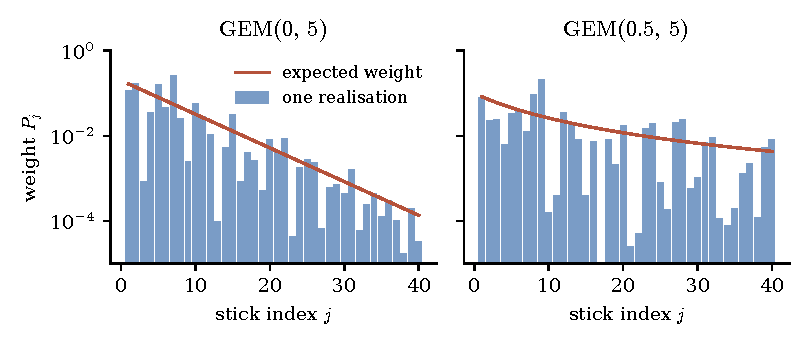
\includegraphics[width=\textwidth]{figures/toolkit_stick.pdf}
\caption{Stick breaking weights $P_j$ on a logarithmic scale for $\GEM(0,5)$ (left) and
$\GEM(0.5,5)$ (right): one realisation (bars) and the expected weights \eqref{toolkit:eq:EP}
(line). With $\alpha=0$ the weights fall geometrically; with $\alpha=1/2$ they fall like a
power of $j$.}
\label{toolkit:fig:stick}
\end{figure}

The last object of this section connects random distributions to random partitions. A random
partition $\Pi$ of $\{1,2,\dots\}$ is exchangeable if its law is invariant under finite
permutations of the integers. Given a sequence $s_1\ge s_2\ge\dots\ge0$ with $\sum_js_j\le1$, the
paintbox partition is formed by painting each integer independently with colour $j$ with
probability $s_j$, or with a unique colour of its own with probability $1-\sum_js_j$, and
grouping integers of the same colour.

\begin{theorem}[Kingman's paintbox]\label{toolkit:thm:paintbox}
Every exchangeable random partition of $\{1,2,\dots\}$ is a mixture of paintbox partitions: there
is a random ranked sequence $S=(S_1,S_2,\dots)$ such that, given $S$, the partition is the paintbox
of $S$. The $S_j$ are the limiting relative frequencies of the blocks, ranked. The Ewens partition
of Section~\ref{toolkit:sec:esf} corresponds to $S\sim\PD(0,\theta)$ and Pitman's to
$S\sim\PD(\alpha,\theta)$ \citep{toolkit:kingman1978,toolkit:pitman1995}.
\end{theorem}

The paintbox plays for partitions the role de Finetti's theorem plays for sequences. In
Chapter~\ref{ch:py} the paint is applied with a nonuniform density, which models ascertainment.

%% ======================================================================
\section{The Ewens and Pitman sampling formulae}\label{toolkit:sec:esf}

This section derives the sampling formula for a neutral sample under the infinite alleles model
from a single predictive rule, records the distribution and moments of the number of alleles,
and extends both to the two parameter family. These are the objects of Part II.

\subsection{The Chinese restaurant and Hoppe's urn}\label{toolkit:sec:crp}

Apply the predictive rule \eqref{toolkit:eq:bm} with a nonatomic $G_0$ and record only which draws
coincide. Customers enter a restaurant one at a time. The first sits at a table. When $m$
customers are seated at $k$ tables with $m_1,\dots,m_k$ at each, the next customer
\begin{equation}\label{toolkit:eq:crp}
\begin{gathered}
\text{starts a new table with probability }\frac{\theta}{\theta+m},\\
\text{joins table }j\text{ with probability }\frac{m_j}{\theta+m}.
\end{gathered}
\end{equation}
\citet{toolkit:hoppe1984} gave the same scheme as an urn: a black ball of weight $\theta$ and
coloured balls of weight one; drawing black adds a ball of a new colour, drawing a colour adds
another of that colour. In genetic terms a table is an allele, the black ball is mutation, and
$\theta=2N\mu$ for a population of $N$ genes ($4N_d\mu$ for $N_d$ diploids).

Write $a_j$ for the number of alleles represented exactly $j$ times among $n$ genes, so that
$\sum_jja_j=n$, and $K_n=\sum_ja_j$ for the number of distinct alleles.

\begin{theorem}[Ewens sampling formula]\label{toolkit:thm:esf}
Under \eqref{toolkit:eq:crp},
\begin{equation}\label{toolkit:eq:esf}
\Prob(a_1,\dots,a_n)=\frac{n!}{(\theta)_n}\prod_{j=1}^n\frac{(\theta/j)^{a_j}}{a_j!}.
\end{equation}
\end{theorem}

\begin{proof}
Fix a seating sequence ending with $k$ tables of sizes $m_1,\dots,m_k$. Its probability is a product
of $n$ factors whose denominators are $\theta,\theta+1,\dots,\theta+n-1$. The numerators are
$\theta$ for each of the $k$ new tables and $1,2,\dots,m_j-1$ for the later arrivals at table $j$,
so the sequence has probability $\theta^k\prod_j(m_j-1)!/(\theta)_n$, whatever the order of
arrivals. The number of ways to partition $n$ labelled genes into blocks with $a_j$ blocks of size
$j$ is $n!/\prod_j(j!)^{a_j}a_j!$. Multiplying, and using $(j-1)!/j!=1/j$, gives
\eqref{toolkit:eq:esf}.
\end{proof}

\citet{toolkit:ewens1972} derived \eqref{toolkit:eq:esf} from the Wright Fisher model with
infinite alleles mutation, \citet{toolkit:antoniak1974} found it as the partition of a Dirichlet
process sample, and Section~\ref{toolkit:sec:coal} derives it a third way, from the coalescent.

\subsection{The number of alleles}\label{toolkit:sec:Kn}

The $(m+1)$st gene is a new allele with probability $\theta/(\theta+m)$, independently of
everything before, so
\begin{equation}\label{toolkit:eq:Kn}
K_n=\sum_{m=0}^{n-1}\xi_m,\qquad \xi_m\sim\mathrm{Bernoulli}\Big(\frac{\theta}{\theta+m}\Big)\
\text{independent},
\end{equation}
and therefore
\begin{equation}\label{toolkit:eq:Kmoments}
\E K_n=\sum_{m=0}^{n-1}\frac{\theta}{\theta+m},\qquad
\Var K_n=\sum_{m=0}^{n-1}\frac{\theta m}{(\theta+m)^2},\qquad
\Prob(K_n=k)=\frac{|s(n,k)|\,\theta^k}{(\theta)_n},
\end{equation}
where $|s(n,k)|$ is the unsigned Stirling number of the first kind, the coefficient of $\theta^k$ in
$(\theta)_n$. For large $n$, $\E K_n=\theta\{\psi(\theta+n)-\psi(\theta)\}\approx\theta\log(1+n/\theta)$,
where $\psi$ is the digamma function, and $K_n/\log n\to\theta$ almost surely \citep{toolkit:korwar1973}.

The factorisation of \eqref{toolkit:eq:esf} into $\theta^{K_n}/(\theta)_n$ times a function of
$a$ alone shows that $K_n$ is sufficient for $\theta$: the configuration given $K_n$ carries no
information about the mutation rate. The maximum likelihood estimator solves
$K_n=\E_\theta K_n$, and since $\Var K_n\approx\theta\log n$ the Fisher information about $\theta$
is only about $\log n/\theta$. Chapters~\ref{ch:esf}, \ref{ch:pig} and \ref{ch:coal} return to
this logarithmic information from three directions.

\begin{example}[All partitions of four genes]\label{toolkit:ex:n4}
There are five allelic configurations of $n=4$ genes. Table~\ref{toolkit:tab:n4} lists their
probabilities under \eqref{toolkit:eq:esf} for $\theta=1$ and $\theta=2$, and under Pitman's
formula of Section~\ref{toolkit:sec:pitman} for $\alpha=1/2$, $\theta=1$; each column sums to one.
At $\theta=1$ the probabilities are $(6,8,3,6,1)/24$, the proportions of permutations of four
objects with each cycle type, because the Ewens formula at $\theta=1$ is the law of the cycle
lengths of a uniform random permutation. For $\theta=2$, the Stirling numbers $|s(4,k)|=6,11,6,1$
give $\Prob(K_4=k)=(0.1,\,0.3667,\,0.4,\,0.1333)$ for $k=1,\dots,4$; four hundred thousand
simulated restaurants give $(0.1002,\,0.3657,\,0.4013,\,0.1328)$. The moments from
\eqref{toolkit:eq:Kmoments} are $\E K_4=77/30=2.567$ and $\Var K_4=641/900=0.712$, and summing
over the table reproduces both exactly. At $\theta=1$, $\E K_4=25/12$ and $\Var K_4=95/144$.
\end{example}

\begin{table}[t]
\centering\small
\caption{Probabilities of the five allelic configurations of $n=4$ genes.}
\label{toolkit:tab:n4}
\begin{tabular}{lcccccc}
\toprule
block sizes & $(a_1,a_2,a_3,a_4)$ & $K_4$ & Ewens $\theta=1$ & Ewens $\theta=2$ & Pitman $(\tfrac12,1)$\\
\midrule
$4$ & $(0,0,0,1)$ & 1 & $1/4$ & $1/10$ & $5/64$\\
$3,1$ & $(1,0,1,0)$ & 2 & $1/3$ & $4/15$ & $3/16$\\
$2,2$ & $(0,2,0,0)$ & 2 & $1/8$ & $1/10$ & $3/64$\\
$2,1,1$ & $(2,1,0,0)$ & 3 & $1/4$ & $2/5$ & $3/8$\\
$1,1,1,1$ & $(4,0,0,0)$ & 4 & $1/24$ & $2/15$ & $5/16$\\
\midrule
$\E K_4$ & & & $25/12$ & $77/30$ & $187/64$\\
\bottomrule
\end{tabular}
\end{table}

\subsection{Pitman's two parameter formula}\label{toolkit:sec:pitman}

The two parameter generalisation changes the restaurant so that large tables are slightly less
attractive and new tables slightly more so the more tables there are. With $0\le\alpha<1$ and
$\theta>-\alpha$, when $m$ customers occupy $k$ tables the next customer
\begin{equation}\label{toolkit:eq:pycrp}
\begin{gathered}
\text{starts a new table with probability }\frac{\theta+k\alpha}{\theta+m},\\
\text{joins table }j\text{ with probability }\frac{m_j-\alpha}{\theta+m}.
\end{gathered}
\end{equation}
The same counting as in Theorem~\ref{toolkit:thm:esf} shows that a particular partition of
$\{1,\dots,n\}$ into blocks of sizes $m_1,\dots,m_k$ has probability
\begin{equation}\label{toolkit:eq:eppf}
p(m_1,\dots,m_k)=\frac{\prod_{i=1}^{k-1}(\theta+i\alpha)}{(\theta+1)_{n-1}}\prod_{j=1}^k(1-\alpha)_{m_j-1},
\end{equation}
Pitman's exchangeable partition probability function \citep{toolkit:pitman1995,toolkit:pitman2006}.
It is symmetric in the block sizes, so the partition is exchangeable; its paintbox is
$\PD(\alpha,\theta)$; and at $\alpha=0$ it reduces to the Ewens formula. The number of blocks has
mean
\begin{equation}\label{toolkit:eq:EKpy}
\E K_n=\frac{\theta}{\alpha}\Big\{\frac{(\theta+\alpha)_n}{(\theta)_n}-1\Big\},\qquad \alpha>0,
\end{equation}
which grows like $n^\alpha$ rather than $\log n$. Indeed $K_n/n^\alpha$ converges almost surely to a
strictly positive random variable, Pitman's $\alpha$ diversity. In Table~\ref{toolkit:tab:n4},
\eqref{toolkit:eq:EKpy} with $\alpha=1/2$, $\theta=1$, $n=4$ gives $187/64=2.92$, larger than
either Ewens column, and the configuration with four singletons is now the second most probable.

\subsection{The logarithmic series and Fisher's alpha}\label{toolkit:sec:logseries}

Fisher's problem was ecological: a sample of $n$ individuals contains $S$ species, of which $a_j$
are represented by exactly $j$ individuals. If species abundances are a Poisson process with
gamma intensity and the number of specimens of each species is Poisson, the expected number of
species seen $j$ times is a negative binomial series, and in the limit of a gamma shape tending to
zero it becomes Fisher's logarithmic series \citep{toolkit:fisher1943}
\begin{equation}\label{toolkit:eq:logseries}
\E a_j=\alpha_F\,\frac{x^j}{j},\qquad x=\frac{n}{n+\alpha_F},\qquad
\E S=\alpha_F\log\Big(1+\frac{n}{\alpha_F}\Big),
\end{equation}
with Fisher's diversity index $\alpha_F$ (not the discount $\alpha$ of the previous subsection).
Under the Ewens formula the expected multiplicities are
\begin{equation}\label{toolkit:eq:EAj}
\E a_j=\frac{\theta}{j}\prod_{i=0}^{j-1}\frac{n-i}{\theta+n-1-i}\;\longrightarrow\;\frac{\theta}{j}
\qquad(n\to\infty,\ j\ \text{fixed}),
\end{equation}
which is \eqref{toolkit:eq:logseries} with $\alpha_F=\theta$ and $x\to1$. Fisher's index is the
Ewens parameter: the logarithmic series is the large sample frequency spectrum of the Ewens
formula, and $\E S$ in \eqref{toolkit:eq:logseries} is the approximation
$\E K_n\approx\theta\log(1+n/\theta)$.

\begin{example}[Williams' Macrolepidoptera]\label{toolkit:ex:williams}
Williams' Rothamsted light trap catch of moths, analysed in \citet{toolkit:fisher1943}, contained
$n=15{,}609$ individuals of $S=240$ species. Solving $S=\alpha_F\log(1+n/\alpha_F)$ gives
Fisher's $\alpha_F=40.25$, and $x=0.99743$. The Ewens maximum likelihood estimate, solving
$240=\theta\{\psi(\theta+n)-\psi(\theta)\}$, is $\hat\theta=40.15$ with standard error $2.84$, the
value used in Chapter~\ref{ch:pig}. The expected numbers of species seen once, twice, three and
ten times are $40.05$, $19.97$, $13.28$ and $3.92$ under \eqref{toolkit:eq:EAj} at $\hat\theta$, and
$40.14$, $20.02$, $13.31$ and $3.92$ under the logarithmic series: the two are indistinguishable at
this sample size. Note that the cruder approximation $\theta\log n=388$ is far from $240$; the
logarithmic growth of $K_n$ sets in only when $n$ is large compared with $\theta$, and here
$n/\theta$ is about $390$.
\end{example}

%% ======================================================================
\section{The Kingman coalescent}\label{toolkit:sec:coal}

The coalescent describes the ancestry of a sample rather than the future of a population. It is
the model behind Part III, and it gives a third derivation of the Ewens formula. This section
derives it from the Wright Fisher model, computes the moments of its height and length, and
superimposes the two mutation models of the neutral theory.

\subsection{Coalescence times}\label{toolkit:sec:coaltimes}

In the neutral Wright Fisher model with $N$ genes, two genes have the same parent in the previous
generation with probability $1/N$. The number of generations back to their common ancestor is
therefore geometric with mean $N$, and measured in units of $N$ generations it converges to an
exponential with mean one. With $k$ genes, the probability that some pair shares a parent is
$\binom k2/N+O(N^{-2})$ and the probability that three or more do, or two pairs at once, is
$O(N^{-2})$. Taking the limit gives Kingman's definition \citep{toolkit:kingman1982}.

\begin{definition}[Kingman coalescent]\label{toolkit:def:coal}
Starting from $n$ lineages, while there are $k\ge2$ lineages each pair merges at rate one,
independently. Thus the time $T_k$ during which there are exactly $k$ lineages is exponential
with rate $\binom k2$, the $T_k$ are independent, and at the end of $T_k$ a uniformly chosen pair
merges. Time is measured in units of $N$ generations ($2N_d$ for a diploid population).
\end{definition}

The height of the tree, the time to the most recent common ancestor, is $H_n=\sum_{k=2}^nT_k$ and
the total branch length is $L_n=\sum_{k=2}^nkT_k$. Since $\E T_k=2/\{k(k-1)\}$ and $\Var
T_k=4/\{k(k-1)\}^2$, and $2/\{k(k-1)\}=2/(k-1)-2/k$ telescopes,
\begin{equation}\label{toolkit:eq:HL}
\begin{gathered}
\E H_n=2\Big(1-\frac1n\Big),\qquad \E L_n=2h_n,\qquad \Var L_n=4b_n,\\
h_n=\sum_{k=1}^{n-1}\frac1k,\qquad b_n=\sum_{k=1}^{n-1}\frac1{k^2}.
\end{gathered}
\end{equation}
Two features deserve comment. The expected height is bounded by two whatever $n$, and more than half of it,
on average, is the time $T_2$ when only two lineages remain: adding genes to a sample adds short
twigs near the present, not depth. The length grows only like $2\log n$, and its variance stays
bounded, so a large sample says little more about the deep tree than a small one. For $n=10$,
$\E H_{10}=1.8$, $\E L_{10}=5.66$ and $\Var L_{10}=6.16$; for $n=100$, $\E H_{100}=1.98$,
$\E L_{100}=10.35$ and $\Var L_{100}=6.54$.

\subsection{Mutation on the tree}\label{toolkit:sec:mutation}

Neutral mutations do not affect the genealogy, so they can be added afterwards. If each gene
mutates with probability $\mu$ per generation, then in units of $N$ generations mutations fall on
each lineage as a Poisson process of rate $\theta/2$, with $\theta=2N\mu$ ($4N_d\mu$ for diploids).

Under the infinite alleles model each mutation creates a new allele. Looking back from the
present, kill a lineage when it meets a mutation, since the allele it carries is then determined.
While $k$ lineages remain, coalescence occurs at rate $k(k-1)/2$ and mutation at rate $k\theta/2$,
so the next event is a mutation with probability $\theta/(\theta+k-1)$. Reading the history
forwards, each added gene is a new allele with probability $\theta/(\theta+k-1)$ and otherwise
copies a uniformly chosen existing gene: this is the Hoppe urn \eqref{toolkit:eq:crp}, and the
sample's allelic partition follows the Ewens formula \eqref{toolkit:eq:esf}.

Under the infinite sites model each mutation strikes a new nucleotide site, so every mutation on
the tree produces one segregating site, and the derived allele at that site is carried by exactly
the sampled genes below the mutated branch. Let $S_n$ be the number of segregating sites and
$\xi_i$ the number of sites at which the derived allele is carried by exactly $i$ of the $n$
genes, $1\le i\le n-1$. The vector $(\xi_1,\dots,\xi_{n-1})$ is the unfolded site frequency
spectrum and $S_n=\sum_i\xi_i$. Figure~\ref{toolkit:fig:coal} shows one realisation.

\begin{figure}[t]
\centering
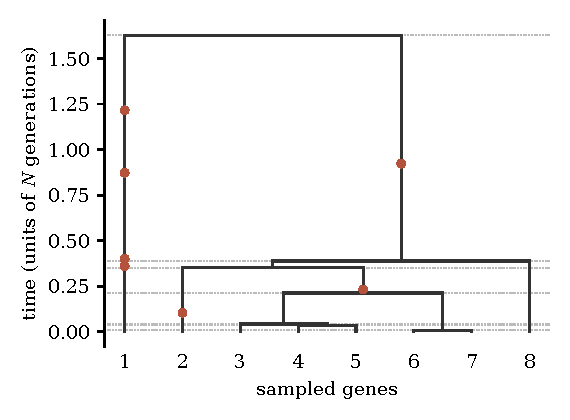
\includegraphics[width=0.72\textwidth]{figures/toolkit_coalescent.pdf}
\caption{A realisation of the Kingman coalescent for $n=8$ genes with infinite sites mutations
at $\theta=3$ (dots). Dotted lines mark the coalescence times. This tree has height $1.63$, total
length $4.30$ and $S=7$ segregating sites, with spectrum $\xi_1=5$, $\xi_5=1$, $\xi_7=1$ and the
remaining $\xi_i=0$; the expected values are $\E H_8=1.75$, $\E L_8=5.19$ and $\E S_8=7.78$.}
\label{toolkit:fig:coal}
\end{figure}

\subsection{Watterson's estimator and the site frequency spectrum}\label{toolkit:sec:watterson}

\begin{theorem}[Segregating sites]\label{toolkit:thm:watterson}
Under the infinite sites model, $S_n\mid L_n\sim\Po(\theta L_n/2)$, and
\begin{equation}\label{toolkit:eq:Smoments}
\E S_n=\theta h_n,\qquad \Var S_n=\theta h_n+\theta^2b_n .
\end{equation}
Watterson's estimator $\hat\theta_W=S_n/h_n$ is unbiased, with variance
$\theta/h_n+\theta^2b_n/h_n^2$ \citep{toolkit:watterson1975}.
\end{theorem}

\begin{proof}
Given the tree, mutations form a Poisson process of rate $\theta/2$ on a set of total length
$L_n$. Then $\E S_n=\tfrac\theta2\E L_n$ and
$\Var S_n=\E\Var(S_n\mid L_n)+\Var\E(S_n\mid L_n)=\tfrac\theta2\E L_n+\tfrac{\theta^2}4\Var L_n$;
substitute \eqref{toolkit:eq:HL}.
\end{proof}

Since $h_n\sim\log n$ while $b_n\to\pi^2/6$, the variance of $\hat\theta_W$ falls only like
$\theta/\log n$, and for moderate samples and large $\theta$ it is dominated by the second term,
$\theta^2b_n/h_n^2$, which comes from the randomness of the single genealogy that all the sites
share. Chapter~\ref{ch:suff}
proves that $S_n$, unlike $K_n$ in the infinite alleles model, is not sufficient for $\theta$, and
Chapter~\ref{ch:coal} gives the exact law of $S_n$ as a sum of independent geometric variables.
Information beyond $S_n$ lies in the spectrum.

\begin{theorem}[Expected spectrum]\label{toolkit:thm:sfs}
Under the infinite sites model, $\E\xi_i=\theta/i$ for $1\le i\le n-1$.
\end{theorem}

\begin{proof}
Let $L_i$ be the total length of branches that subtend exactly $i$ sampled genes, so
$\E\xi_i=\tfrac\theta2\E L_i$. During the epoch with $k$ lineages, the numbers of sampled genes
descending from the $k$ lineages form a random composition of $n$ into $k$ positive parts. By the
P\'olya urn argument of Proposition~\ref{toolkit:prop:polya} applied to the forward history,
with $k$ colours each starting with one ball, every composition is equally likely, so a given
lineage subtends exactly $i$ genes with probability
$\binom{n-i-1}{k-2}\big/\binom{n-1}{k-1}$. Hence
\[
\E L_i=\sum_{k=2}^{n-i+1}k\,\E T_k\,\frac{\binom{n-i-1}{k-2}}{\binom{n-1}{k-1}}
=\sum_{k=2}^{n-i+1}\frac{2}{k-1}\,\frac{\binom{n-i-1}{k-2}}{\binom{n-1}{k-1}} .
\]
Writing $j=k-2$ and expanding the binomials, the summand is
$2\,(n-i-1)!\,(i-1)!\,\binom{n-2-j}{i-1}/(n-1)!$, and the hockey stick identity
$\sum_{j=0}^{n-i-1}\binom{n-2-j}{i-1}=\binom{n-1}{i}$ gives
$\E L_i=2\,(n-i-1)!\,(i-1)!\,\binom{n-1}{i}/(n-1)!=2/i$.
\end{proof}

The spectrum is a decreasing harmonic sequence: singletons are the most common class, and the
expected number of sites at frequency $i/n$ is inversely proportional to $i$. It is the infinite
sites counterpart of \eqref{toolkit:eq:EAj}, and the departures of observed spectra from $\theta/i$
are the basis of the neutrality tests of Tajima and of Fu and Li \citep{toolkit:fu1995}. Summing
over $i$ recovers $\E S_n=\theta h_n$.

\begin{example}[Five genes]\label{toolkit:ex:sfs}
For $n=5$ and $\theta=2$ the theory gives $\E(\xi_1,\xi_2,\xi_3,\xi_4)=(2,1,0.667,0.5)$,
$\E S_5=2h_5=4.167$, $\Var S_5=2h_5+4b_5=9.861$, $\E H_5=1.6$ and $\E L_5=4.167$. One hundred
thousand simulated coalescent trees give spectrum means $(2.010,0.998,0.669,0.501)$, $\E S=4.178$,
$\Var S=9.854$, $\E H=1.603$ and $\E L=4.175$. The probability that the sample is monomorphic is
$\prod_{k=2}^5(k-1)/(k-1+\theta)=1/15=0.0667$, against $0.0669$ in simulation; this product form
is the first instance of the geometric decomposition of Chapter~\ref{ch:coal}.
\end{example}

\begin{example}[Kreitman's alcohol dehydrogenase sample]\label{toolkit:ex:kreitman}
Kreitman's survey of the \emph{Adh} locus of \emph{Drosophila melanogaster}
\citep{toolkit:kreitman1983} sequenced $n=11$ alleles and found $S=43$ segregating sites. With
$h_{11}=2.929$ and $b_{11}=1.550$, Watterson's estimate for the region is
$\hat\theta_W=43/2.929=14.7$. At that value the standard deviation of $S$ is
$\sqrt{14.7\cdot2.929+14.7^2\cdot1.550}=19.4$, so the standard error of $\hat\theta_W$ is about
$6.6$: the coefficient of variation is forty five percent, and almost all of it comes from the
term $\theta^2b_n$, the variability of the genealogy itself. Sequencing more alleles would barely
help; sequencing more independent loci would. Under neutrality the expected spectrum at
$\hat\theta_W$ is $14.7/i$, that is $14.7$ singletons, $7.3$ doubletons and so on down to $1.5$
sites at frequency $10/11$.
\end{example}

%% ======================================================================
\section{Bayesian tools}\label{toolkit:sec:bayes}

This section collects the Bayesian devices used in the later chapters: scale mixtures of normals,
the horseshoe prior and its shrinkage weight, and three data augmentation identities that turn
awkward likelihoods into conditionally conjugate ones. It closes with a paragraph on the large
sample behaviour of posteriors.

\subsection{Scale mixtures of normals}\label{toolkit:sec:scalemix}

A random variable $\beta$ is a scale mixture of normals if $\beta=\sqrt V\,Z$ with $Z\sim
\mathcal{N}(0,1)$ independent of a positive $V$, so that
$p(\beta)=\int\mathcal{N}(\beta;0,v)\,p(v)\,\dd v$. The class is closed under the operations Bayesian
computation needs: given $V$ everything is Gaussian, and $V$ is updated by a one dimensional
draw. Two classical members are the Student $t_\nu$, for which $1/V\sim\Ga(\nu/2,\nu/2)$, and the
Laplace distribution with scale $b$, for which $V$ is exponential with mean $2b^2$
\citep{toolkit:andrews1974}. Numerically, at $\beta=1.3$ the $t_3$ density $0.150389$ and the
Laplace density $0.136266$ (with $b=1$) are both reproduced to six decimals by integrating the
normal density against the mixing law.

\subsection{Global local shrinkage and the horseshoe}\label{toolkit:sec:horseshoe}

In a sparse normal means problem, $y_i\mid\beta_i\sim\mathcal{N}(\beta_i,\sigma^2)$ for
$i=1,\dots,p$, and most $\beta_i$ are near zero while a few are large. A global local prior is a
scale mixture with one scale shared by all coordinates and one particular to each:
\begin{equation}\label{toolkit:eq:gl}
\beta_i\mid\lambda_i,\tau\sim\mathcal{N}(0,\lambda_i^2\tau^2\sigma^2),\qquad
\lambda_i\sim\pi(\lambda_i),\qquad \tau\sim\pi(\tau).
\end{equation}
The global scale $\tau$ adapts to the overall level of sparsity; the local scales $\lambda_i$ let
individual signals escape it. The horseshoe of \citet{toolkit:carvalho2010} takes
$\lambda_i\sim\mathrm{C}^+(0,1)$, the half Cauchy distribution with density
$2/\{\pi(1+\lambda^2)\}$ on $(0,\infty)$.

Given the scales the posterior mean is linear, and the shrinkage weight
\begin{equation}\label{toolkit:eq:kappa}
\kappa_i=\frac{1}{1+\lambda_i^2\tau^2}\in(0,1),\qquad
\E[\beta_i\mid y_i,\lambda_i,\tau]=(1-\kappa_i)\,y_i,
\end{equation}
is the fraction of the observation that is shrunk away. Integrating over $\lambda_i$,
$\E[\beta_i\mid y_i,\tau]=\{1-\E(\kappa_i\mid y_i,\tau)\}y_i$, so the whole behaviour of the prior is
carried by the law of $\kappa_i$.

\begin{proposition}[The horseshoe weight]\label{toolkit:prop:kappa}
With $\tau=\sigma=1$ and $\lambda\sim\mathrm{C}^+(0,1)$, the weight $\kappa=1/(1+\lambda^2)$ has the
$\Be(1/2,1/2)$ distribution, and its posterior given $y$ has density proportional to
$(1-\kappa)^{-1/2}e^{-\kappa y^2/2}$ on $(0,1)$. For general $\tau$,
$\Prob(\kappa<1/2)=(2/\pi)\arctan\tau$.
\end{proposition}

\begin{proof}
Since $\lambda=\{(1-\kappa)/\kappa\}^{1/2}$, $|\dd\lambda/\dd\kappa|=\tfrac12\kappa^{-3/2}(1-\kappa)^{-1/2}$
and $1+\lambda^2=1/\kappa$, the density of $\kappa$ is
$\{2\kappa/\pi\}\cdot\tfrac12\kappa^{-3/2}(1-\kappa)^{-1/2}=\kappa^{-1/2}(1-\kappa)^{-1/2}/\pi$, the
$\Be(1/2,1/2)$ density. Given $\kappa$, $y\sim\mathcal{N}(0,1+\lambda^2)=\mathcal{N}(0,1/\kappa)$, so
the likelihood of $\kappa$ is $\kappa^{1/2}e^{-\kappa y^2/2}$; multiply by the prior. Finally
$\kappa<1/2$ if and only if $\lambda\tau>1$, which has probability $1-(2/\pi)\arctan(1/\tau)
=(2/\pi)\arctan\tau$.
\end{proof}

The $\Be(1/2,1/2)$ density is unbounded at both ends, the horseshoe shape that names the prior:
it expects each coordinate to be either almost entirely noise ($\kappa$ near one) or almost
entirely signal ($\kappa$ near zero). Chapter~\ref{ch:ftns} reads Fisher's additive model as the
hypothesis $\kappa=1$, and Chapter~\ref{ch:mp} identifies $\kappa$ with the first stick of a
$\GEM$ sequence. The marginal prior density of $\beta$ has no closed form but satisfies, with
$c_0=(2\pi^3)^{-1/2}$,
\begin{equation}\label{toolkit:eq:hsbounds}
\tfrac {c_0}2\log\Big(1+\frac4{\beta^2}\Big)<p(\beta)<c_0\log\Big(1+\frac2{\beta^2}\Big),
\end{equation}
so it has a logarithmic pole at zero and Cauchy tails \citep{toolkit:carvalho2010}. At
$\beta=0.1$, $1$ and $3$ the density is $0.603$, $0.117$ and $0.0237$, inside the bounds
$(0.381,0.673)$, $(0.102,0.140)$ and $(0.0233,0.0255)$.

\begin{example}[How the horseshoe shrinks]\label{toolkit:ex:hs}
With $\tau=\sigma=1$, the posterior means of $\kappa$ and of $\beta$ for several observations are
\begin{center}\small
\begin{tabular}{lccccccc}
\toprule
$y$ & 0 & 0.5 & 1 & 2 & 3 & 5 & 10\\
\midrule
$\E(\kappa\mid y)$ & 0.667 & 0.655 & 0.620 & 0.469 & 0.263 & 0.084 & 0.020\\
$\E(\beta\mid y)$ & 0 & 0.172 & 0.380 & 1.063 & 2.210 & 4.579 & 9.798\\
\bottomrule
\end{tabular}
\end{center}
At $y=0$, $\E(\kappa\mid y)=B(2,\tfrac12)/B(1,\tfrac12)=2/3$ exactly. Small observations are
shrunk by about two thirds, large ones are left almost alone: the bias at $y=10$ is $0.20$, and it
tends to zero as $y$ grows. A normal prior with the same shrinkage at the origin would shrink
every observation by the same fraction. With a small global scale the prior becomes more
sceptical: at $\tau=0.1$ the prior probability that $\kappa<1/2$ is only $0.063$.
\end{example}

\subsection{Beta augmentation of Gamma ratios}\label{toolkit:sec:betaaug}

Concentration parameters such as the Ewens $\theta$ enter likelihoods through ratios
$\Gamma(\theta)/\Gamma(\theta+n)=1/(\theta)_n$, which block conjugate updating. The Beta integral
removes the block:
\begin{equation}\label{toolkit:eq:betaaug}
\frac{\Gamma(\theta)}{\Gamma(\theta+n)}=\frac{1}{\Gamma(n)}\int_0^1\eta^{\theta-1}(1-\eta)^{n-1}\,\dd\eta,
\end{equation}
which is $B(\theta,n)=\Gamma(\theta)\Gamma(n)/\Gamma(\theta+n)$ rearranged. For the Ewens likelihood
$\theta^{K}/(\theta)_n$ with a $\Ga(a_0,b_0)$ prior, introduce $\eta$ with joint density
proportional to $\theta^{K+a_0-1}e^{-b_0\theta}\eta^{\theta-1}(1-\eta)^{n-1}$. Both conditionals are
standard:
\begin{equation}\label{toolkit:eq:ewgibbs}
\eta\mid\theta\sim\Be(\theta,n),\qquad \theta\mid\eta\sim\Ga(K+a_0,\;b_0-\log\eta),
\end{equation}
a variant of the sampler of \citet{toolkit:escobar1995}, who augment with $\Be(\theta+1,n)$ and obtain a two component Gamma mixture for $\theta$. Chapter~\ref{ch:pig} uses this variant throughout and
Chapter~\ref{ch:rc} develops the general theory of priors for such ratios.

\begin{example}[A small Ewens posterior]\label{toolkit:ex:betaaug}
At $\theta=2.5$ and $n=10$ both sides of \eqref{toolkit:eq:betaaug} equal $9.714\times10^{-9}$. Take
a sample of $n=30$ genes with $K=8$ alleles and the prior $\Ga(1,0.2)$, an exponential with mean
five. Fifty eight thousand iterations of \eqref{toolkit:eq:ewgibbs} give posterior mean $3.61$ and
standard deviation $1.61$; numerical integration of the exact posterior
$\propto\theta^{8}e^{-0.2\theta}/(\theta)_{30}$ gives $3.616$ and $1.592$. The same posterior is
the target of the likelihood free methods of Section~\ref{toolkit:sec:lfi}.
\end{example}

\subsection{P\'olya Gamma and P\'olya inverse gamma}\label{toolkit:sec:pg}

Two further identities are stated here for reference; both are proved in the papers cited.

A random variable $\omega$ has the P\'olya Gamma distribution $\PG(b,c)$, $b>0$, $c\in\R$, if
\[
\omega\overset{d}{=}\frac{1}{2\pi^2}\sum_{k=1}^\infty\frac{g_k}{(k-1/2)^2+c^2/(4\pi^2)},\qquad
g_k\sim\Ga(b,1)\ \text{independent}.
\]
\citet{toolkit:polson2013} prove that for $a\in\R$ and $h=a-b/2$,
\begin{equation}\label{toolkit:eq:pg}
\frac{(e^{\psi})^a}{(1+e^{\psi})^b}=2^{-b}e^{h\psi}\int_0^\infty e^{-\omega\psi^2/2}\,p(\omega\mid b,0)\,\dd\omega,
\end{equation}
that $\E[e^{-t\omega}]=\cosh^{-b}(\sqrt{t/2})$ for $\omega\sim\PG(b,0)$, that
$\E\omega=\{b/(2c)\}\tanh(c/2)$ for $\omega\sim\PG(b,c)$, and that $\omega\mid\psi\sim\PG(b,\psi)$
under the joint density implied by \eqref{toolkit:eq:pg}. The logistic and negative binomial
likelihoods are of the form on the left with $\psi$ linear in the regression coefficients, so
given $\omega$ the likelihood is Gaussian in $\psi$. As checks, the product
$\prod_k\{1+t/(2\pi^2(k-1/2)^2)\}^{-b}$ truncated at two hundred thousand terms equals
$\cosh^{-1}(\sqrt{0.35})=0.847340$ at $b=1$, $t=0.7$, and the series mean of $\PG(1,1.5)$ is
$0.21172=\tanh(0.75)/3$.

The P\'olya inverse gamma law of \citet{toolkit:he2022} handles a parameter that appears in a
reciprocal Gamma function. A positive random variable $X_0$ has the $\mathrm{PIG}(0)$ law if
\begin{equation}\label{toolkit:eq:pig}
\E\big[e^{-s^2X_0}\big]=\frac{e^{-\gamma s}}{\Gamma(1+s)},\qquad s>0,
\end{equation}
with $\gamma$ the Euler Mascheroni constant, so that $1/\Gamma(1+s)=e^{\gamma s}\E[e^{-s^2X_0}]$
is Gaussian in $s$ given $X_0$. The law is an infinite convolution of scaled inverse gamma
variables and has mean $\pi^2/12$. Chapter~\ref{ch:pig} uses \eqref{toolkit:eq:betaaug} for
Fisher's richness parameter and \eqref{toolkit:eq:pig} for his shape parameter.

\subsection{Bernstein and von Mises}\label{toolkit:sec:bvm}

In a regular parametric model with a prior that is continuous and positive at the true value
$\theta_0$, the posterior is asymptotically normal, centred at the maximum likelihood estimator,
with variance the inverse of the Fisher information: the total variation distance between
$\pi(\theta\mid y_{1:n})$ and $\mathcal{N}(\hat\theta_n,I_n(\hat\theta_n)^{-1})$ tends to zero in
probability \citep{toolkit:vandervaart1998}. Bayesian and likelihood intervals then agree to first
order, and the prior is forgotten. What matters in genetics is the rate at which $I_n$ grows. For
the Ewens parameter it grows like $\log n/\theta$, not $n$, so the effective sample size is the
number of alleles $K_n$, and the approximation is accurate only when $K_n$ is large; for the
small and hyperdiverse samples of Chapter~\ref{ch:pig}, and for the many parameter regressions of
Part I where the number of parameters grows with $n$, the theorem does not apply and the prior
matters.

%% ======================================================================
\section{Likelihood free inference}\label{toolkit:sec:lfi}

Coalescent models are easy to simulate and hard to evaluate: the likelihood of a sample is an
integral over all genealogies. This section describes the two responses used in Part III,
rejection approximate Bayesian computation and quantile regression on simulations, and the lemma
that justifies the second.

\subsection{Rejection ABC}\label{toolkit:sec:abc}

Let $\pi(\theta)$ be a prior, $p(y\mid\theta)$ a model that can be simulated, $S$ a summary
statistic, $\rho$ a distance and $\epsilon\ge0$ a tolerance. Rejection approximate Bayesian
computation \citep{toolkit:tavare1997,toolkit:pritchard1999,toolkit:beaumont2002} repeats:
draw $\theta\sim\pi$; draw $y\sim p(\cdot\mid\theta)$; keep $\theta$ if
$\rho(S(y),S(y_{\mathrm{obs}}))\le\epsilon$.

\begin{proposition}[What rejection ABC computes]\label{toolkit:prop:abc}
The accepted values are independent draws from
$\pi\{\theta\mid\rho(S(Y),S(y_{\mathrm{obs}}))\le\epsilon\}$. If $S$ is discrete and $\epsilon=0$
this is $\pi(\theta\mid S(Y)=S(y_{\mathrm{obs}}))$, and if moreover $S$ is sufficient it is the exact
posterior $\pi(\theta\mid y_{\mathrm{obs}})$.
\end{proposition}

\begin{proof}
The pair $(\theta,Y)$ is drawn from the joint law, and accepting on an event $E$ of positive
probability yields the conditional law of $\theta$ given $E$. With $\epsilon=0$ the event is
$\{S(Y)=s_{\mathrm{obs}}\}$, and sufficiency means $\pi(\theta\mid y)$ depends on $y$ only through
$S(y)$.
\end{proof}

The two defects of the method are visible in the statement: the analyst must choose $S$, and
unless $S$ is sufficient the target is not the posterior; and the analyst must choose $\epsilon$,
and a positive $\epsilon$ conditions on a larger event, which inflates the spread.

\begin{example}[ABC for the Ewens parameter]\label{toolkit:ex:abc}
Return to $n=30$, $K=8$ and the prior $\Ga(1,0.2)$ of Example~\ref{toolkit:ex:betaaug}. Since $K_n$
is sufficient, rejection with $S=K_n$ and $\epsilon=0$ is exact. Of two hundred thousand
simulations, using the Bernoulli representation \eqref{toolkit:eq:Kn}, $7.0$ percent are accepted;
the accepted values have mean $3.61$ and standard deviation $1.60$, and $5$, $50$ and $95$
percent quantiles $1.55$, $3.34$ and $6.65$, against the exact $3.616$, $1.592$ and $1.555$,
$3.345$, $6.599$. Widening the tolerance to $|K-8|\le2$ raises the acceptance rate to $34$ percent
but inflates the standard deviation to $1.89$, an error that more simulation does not remove.
\end{example}

\subsection{The check loss and quantile regression}\label{toolkit:sec:check}

For $u\in(0,1)$ the check loss is $\rho_u(z)=z\{u-\one(z<0)\}$: it charges $u|z|$ for an
underestimate and $(1-u)|z|$ for an overestimate. Quantile regression \citep{toolkit:koenker1978}
minimises it.

\begin{lemma}[The check loss identifies quantiles]\label{toolkit:lem:check}
Let $X$ be a real random variable with $\E|X|<\infty$ and distribution function $F$. Then
$c\mapsto\E\rho_u(X-c)$ is convex and minimised exactly at the $u$ quantiles of $X$, that is at
the $c$ with $F(c-)\le u\le F(c)$. Consequently, for a pair $(\theta,Y)$ with $\E|\theta|<\infty$,
the minimiser over measurable functions $h$ of $\E\rho_u(\theta-h(Y))$ is the conditional quantile
$h(y)=F^{-1}_{\theta\mid Y=y}(u)$ for almost every $y$.
\end{lemma}

\begin{proof}
Convexity holds because $\rho_u$ is convex. Writing $\rho_u(z)=uz^+ +(1-u)z^-$ and differentiating
under the expectation, the right derivative of $c\mapsto\E\rho_u(X-c)$ is
$-u\Prob(X>c)+(1-u)\Prob(X\le c)=F(c)-u$, and the left derivative is $F(c-)-u$. A convex function
is minimised where the left derivative is at most zero and the right derivative at least zero.
For the conditional statement, apply the first part to the conditional law of $\theta$ given
$Y=y$ and integrate over $y$.
\end{proof}

Fitting $h$ for one $u$ gives one conditional quantile; letting $u$ be an input, as
Chapter~\ref{ch:suff} does, gives the whole conditional quantile function, and so the whole
posterior, from simulated pairs $(\theta_i,y_i)$ alone. Least squares returns one number per $y$;
the check loss, integrated over $u$, returns a law.

\begin{example}[Posterior quantiles by regression]\label{toolkit:ex:qr}
On one thousand and one standard normal draws, minimising $\sum\rho_u(z_i-c)$ over $c$ returns the
empirical $u$ quantile exactly for $u=0.1$, $0.5$ and $0.9$. For the Ewens problem, simulate six
thousand pairs $(\theta_i,K_i)$ from the prior and the model with $n=30$, and fit for each $u$ the
linear quantile regression of $\log\theta$ on $(1,\log K,\log^2K)$ by linear programming; since
$\log$ is increasing, quantiles of $\log\theta$ exponentiate to quantiles of $\theta$. At
$K=3$, $8$ and $15$ the fitted $5$, $50$ and $95$ percent quantiles are
\begin{center}\small
\begin{tabular}{lccc}
\toprule
& $K=3$ & $K=8$ & $K=15$\\
\midrule
$u=0.05$, fitted (exact) & 0.208 (0.239) & 1.564 (1.555) & 5.174 (5.266)\\
$u=0.50$, fitted (exact) & 0.815 (0.839) & 3.402 (3.345) & 9.621 (9.573)\\
$u=0.95$, fitted (exact) & 2.158 (2.217) & 6.820 (6.599) & 16.954 (16.758)\\
\bottomrule
\end{tabular}
\end{center}
One regression per quantile level, trained once, answers every data set, with no tolerance and no
rejection; the error, at most about three percent except in the lower tail, is an estimation error
that shrinks with the simulation budget and the flexibility of the basis.
\end{example}

\subsection{Noise outsourcing}\label{toolkit:sec:noise}

The last result says that the posterior is not merely approximable by a function of the data and
an independent uniform variable, but is one.

\begin{theorem}[Noise outsourcing]\label{toolkit:thm:noise}
Let $(\theta,Y)$ be a random element of $\Theta\times\mathcal{Y}$, with $\Theta$ standard Borel.
There are a measurable map $H:(0,1)\times\mathcal{Y}\to\Theta$ and a random variable
$U\sim\mathrm{Unif}(0,1)$ independent of $Y$ such that $\theta=H(U,Y)$ almost surely. When
$\Theta\subseteq\R$ one may take $H(u,y)=F^{-1}_{\theta\mid Y=y}(u)$
\citep[Theorem~6.10]{toolkit:kallenberg2002}.
\end{theorem}

\begin{proof}[Sketch]
Take $\Theta=\R$; a standard Borel space is Borel isomorphic to a Borel subset of $\R$, which
reduces the general case to this one. Let $F_y$ be a regular version of the conditional
distribution function of $\theta$ given $Y=y$, and let $V\sim\mathrm{Unif}(0,1)$ be independent of
$(\theta,Y)$. Define $U=F_Y(\theta-)+V\{F_Y(\theta)-F_Y(\theta-)\}$, which randomises within any
atom. Given $Y=y$, $U$ is uniform on $(0,1)$ (the probability integral transform, randomised at
atoms), so $U$ is uniform and independent of $Y$. And $F_y^{-1}(U)=\theta$ almost surely, because
$U$ lies in $[F_y(\theta-),F_y(\theta)]$ and the quantile function maps that interval back to
$\theta$ except on a null set.
\end{proof}

Read together with Lemma~\ref{toolkit:lem:check}, the theorem says that the posterior is the map
$u\mapsto H(u,y_{\mathrm{obs}})$, that this map minimises an expected check loss over simulated
pairs, and that it can therefore be learned by regression. Chapter~\ref{ch:suff} builds the
method on this observation and shows that a learned map with a low dimensional bottleneck that
attains the Bayes risk certifies a sufficient statistic, and Chapter~\ref{ch:coal} applies it to
the coalescent.

%% ======================================================================
\section{Exercises}\label{toolkit:sec:exercises}

\begin{enumerate}[label=\arabic*.,leftmargin=*,itemsep=4pt]
\item Show that for a biallelic locus with genotype frequencies $(P_{11},P_{12},P_{22})$ one
generation of random mating gives Hardy Weinberg proportions, and that the inbreeding coefficient
$F$ of \eqref{toolkit:eq:F} satisfies $F=(P_{11}P_{22}-P_{12}^2/4)/(pq)$.
\emph{Hint.} Expand $P_{11}P_{22}$ using \eqref{toolkit:eq:F}.

\item With three alleles at frequencies $(0.5,0.3,0.2)$, compute the Hardy Weinberg genotype
frequencies and the expected heterozygosity $1-\sum_ip_i^2$. What is the dimension of the
Hardy Weinberg manifold inside the simplex of genotype frequencies?
\emph{Hint.} The heterozygosity is $0.62$; count free parameters on each side.

\item Prove that $|D|\le\tfrac14$ for any two biallelic loci, and find the haplotype frequencies
that attain it. \emph{Hint.} $D=x_{AB}x_{ab}-x_{Ab}x_{aB}\le x_{AB}x_{ab}$ and
$x_{AB}+x_{ab}\le1$.

\item In Example~\ref{toolkit:ex:avg}, let $p$ vary in $(0,1)$ with the genotypic values fixed.
Plot $\sigma^2_A(p)$ and $\sigma^2_D(p)$, and show that $\sigma^2_A$ is largest at
$p=(7-\sqrt{17})/8\approx0.360$, where it equals $4.957$, while $\sigma^2_D$ is largest at $p=1/2$.
\emph{Hint.} $\sigma^2_A=8p(1-p)(2-p)^2$, whose derivative is $8(2-p)(4p^2-7p+2)$.

\item For the neutral Wright Fisher model with $N$ genes, show that
$\E[x_t(1-x_t)]=(1-1/N)^tx_0(1-x_0)$ and deduce that the probability that the population is still
polymorphic at time $t$ is at least $4(1-1/N)^tx_0(1-x_0)$. For $N=20$ and $x_0=1/2$, how
long is the population guaranteed to stay polymorphic with probability at least one half?
\emph{Hint.} $x(1-x)\le\tfrac14$ on the event of polymorphism and is zero otherwise.

\item Solve $\mathcal{L}T=-1$ with $T(0)=T(1)=0$ for the neutral diffusion and show that the mean
absorption time of a new mutant, $x=1/N$, is about $2(1+\log N)$ generations, while conditional
on fixation it is about $2N$ generations. \emph{Hint.} For the conditional time solve
$\mathcal{L}(uT^*)=-u$ with $u(x)=x$.

\item Using Proposition~\ref{toolkit:prop:dir}(i), show that if $P\sim\Dir(a_1,\dots,a_k)$ then
$P_1/(P_1+P_2)\sim\Be(a_1,a_2)$ independently of $P_1+P_2$. Check numerically for $a=(1,2,3)$.
\emph{Hint.} The ratio involves only $G_1$ and $G_2$.

\item Prove \eqref{toolkit:eq:EP} and deduce that for $\alpha=0$ the number of sticks needed to
leave expected mass below $\epsilon$ is about $\log(1/\epsilon)/\log(1+1/\theta)$. Compare with
the value $26$ found in Example~\ref{toolkit:ex:stick}. \emph{Hint.} Independence of the $W_j$ gives
$\E\prod(1-W_j)=\prod\E(1-W_j)$.

\item Enumerate the seven configurations of $n=5$ genes, compute their Ewens probabilities at
$\theta=1$, and check that they are the cycle type proportions of the symmetric group on five
letters. \emph{Hint.} The numbers of permutations are $1,10,15,20,20,30,24$.

\item Show that $\E K_n$ in \eqref{toolkit:eq:EKpy} tends to the Ewens value
$\sum_{m<n}\theta/(\theta+m)$ as $\alpha\to0$. \emph{Hint.} Write
$(\theta+\alpha)_n/(\theta)_n=\prod_m(1+\alpha/(\theta+m))$ and expand to first order in $\alpha$.

\item Show that $\E T_2/\E H_n\to1/2$ as $n\to\infty$, and that $\Var H_n\to\tfrac43\pi^2-12
\approx1.16$. \emph{Hint.} $\Var H_n=\sum_k4/\{k(k-1)\}^2$; use partial fractions.

\item Write a rejection ABC sampler for $\theta$ from Watterson's $S$ with $n=11$, $S=43$ and a
flat prior on $(0,60)$, and compare the accepted values with the exact posterior obtained from
the geometric representation of Chapter~\ref{ch:coal}. \emph{Hint.} Simulate the $T_k$ of Definition~\ref{toolkit:def:coal}, form $L_n$, and then draw
$S\sim\Po(\theta L_n/2)$.
\end{enumerate}

\begin{thebibliography}{99}

\bibitem[Aldous(1985)]{toolkit:aldous1985}
Aldous, D.~J. (1985). Exchangeability and related topics. In \emph{\'Ecole d'\'Et\'e de
Probabilit\'es de Saint Flour XIII}, Lecture Notes in Mathematics 1117, 1 to 198. Berlin:
Springer.

\bibitem[Andrews and Mallows(1974)]{toolkit:andrews1974}
Andrews, D.~F. and Mallows, C.~L. (1974). Scale mixtures of normal distributions.
\emph{Journal of the Royal Statistical Society, Series B} 36, 99 to 102.

\bibitem[Antoniak(1974)]{toolkit:antoniak1974}
Antoniak, C.~E. (1974). Mixtures of Dirichlet processes with applications to Bayesian
nonparametric problems. \emph{The Annals of Statistics} 2, 1152 to 1174.

\bibitem[Beaumont et~al.(2002)]{toolkit:beaumont2002}
Beaumont, M.~A., Zhang, W. and Balding, D.~J. (2002). Approximate Bayesian computation in
population genetics. \emph{Genetics} 162, 2025 to 2035.

\bibitem[Blackwell and MacQueen(1973)]{toolkit:blackwell1973}
Blackwell, D. and MacQueen, J.~B. (1973). Ferguson distributions via P\'olya urn schemes.
\emph{The Annals of Statistics} 1, 353 to 355.

\bibitem[Carvalho et~al.(2010)]{toolkit:carvalho2010}
Carvalho, C.~M., Polson, N.~G. and Scott, J.~G. (2010). The horseshoe estimator for sparse
signals. \emph{Biometrika} 97, 465 to 480.

\bibitem[Diaconis and Freedman(1980)]{toolkit:diaconis1980}
Diaconis, P. and Freedman, D. (1980). Finite exchangeable sequences. \emph{The Annals of
Probability} 8, 745 to 764.

\bibitem[Escobar and West(1995)]{toolkit:escobar1995}
Escobar, M.~D. and West, M. (1995). Bayesian density estimation and inference using mixtures.
\emph{Journal of the American Statistical Association} 90, 577 to 588.

\bibitem[Ewens(1972)]{toolkit:ewens1972}
Ewens, W.~J. (1972). The sampling theory of selectively neutral alleles. \emph{Theoretical
Population Biology} 3, 87 to 112.

\bibitem[Ewens(2004)]{toolkit:ewens2004}
Ewens, W.~J. (2004). \emph{Mathematical Population Genetics I: Theoretical Introduction}, second
edition. New York: Springer.

\bibitem[Ferguson(1973)]{toolkit:ferguson1973}
Ferguson, T.~S. (1973). A Bayesian analysis of some nonparametric problems. \emph{The Annals of
Statistics} 1, 209 to 230.

\bibitem[Fisher(1918)]{toolkit:fisher1918}
Fisher, R.~A. (1918). The correlation between relatives on the supposition of Mendelian
inheritance. \emph{Transactions of the Royal Society of Edinburgh} 52, 399 to 433.

\bibitem[Fisher(1941)]{toolkit:fisher1941}
Fisher, R.~A. (1941). Average excess and average effect of a gene substitution. \emph{Annals of
Eugenics} 11, 53 to 63.

\bibitem[Fisher et~al.(1943)]{toolkit:fisher1943}
Fisher, R.~A., Corbet, A.~S. and Williams, C.~B. (1943). The relation between the number of
species and the number of individuals in a random sample of an animal population. \emph{Journal
of Animal Ecology} 12, 42 to 58.

\bibitem[Ford(1971)]{toolkit:ford1971}
Ford, E.~B. (1971). \emph{Ecological Genetics}, third edition. London: Chapman and Hall.

\bibitem[Fu(1995)]{toolkit:fu1995}
Fu, Y.~X. (1995). Statistical properties of segregating sites. \emph{Theoretical Population
Biology} 48, 172 to 197.

\bibitem[He et~al.(2019)]{toolkit:he2022}
He, J., Polson, N.~G. and Xu, J. (2019). Data augmentation with P\'olya inverse gamma.
arXiv:1905.12141.

\bibitem[Heath and Sudderth(1976)]{toolkit:heath1976}
Heath, D. and Sudderth, W. (1976). De Finetti's theorem on exchangeable variables. \emph{The
American Statistician} 30, 188 to 189.

\bibitem[Hoppe(1984)]{toolkit:hoppe1984}
Hoppe, F.~M. (1984). P\'olya like urns and the Ewens sampling formula. \emph{Journal of
Mathematical Biology} 20, 91 to 94.

\bibitem[Kallenberg(2002)]{toolkit:kallenberg2002}
Kallenberg, O. (2002). \emph{Foundations of Modern Probability}, second edition. New York:
Springer.

\bibitem[Kimura(1962)]{toolkit:kimura1962}
Kimura, M. (1962). On the probability of fixation of mutant genes in a population.
\emph{Genetics} 47, 713 to 719.

\bibitem[Kingman(1978)]{toolkit:kingman1978}
Kingman, J.~F.~C. (1978). The representation of partition structures. \emph{Journal of the London
Mathematical Society} 18, 374 to 380.

\bibitem[Kingman(1982)]{toolkit:kingman1982}
Kingman, J.~F.~C. (1982). The coalescent. \emph{Stochastic Processes and their Applications} 13,
235 to 248.

\bibitem[Koenker and Bassett(1978)]{toolkit:koenker1978}
Koenker, R. and Bassett, G. (1978). Regression quantiles. \emph{Econometrica} 46, 33 to 50.

\bibitem[Korwar and Hollander(1973)]{toolkit:korwar1973}
Korwar, R.~M. and Hollander, M. (1973). Contributions to the theory of Dirichlet processes.
\emph{The Annals of Probability} 1, 705 to 711.

\bibitem[Kreitman(1983)]{toolkit:kreitman1983}
Kreitman, M. (1983). Nucleotide polymorphism at the alcohol dehydrogenase locus of
\emph{Drosophila melanogaster}. \emph{Nature} 304, 412 to 417.

\bibitem[Pitman(1995)]{toolkit:pitman1995}
Pitman, J. (1995). Exchangeable and partially exchangeable random partitions. \emph{Probability
Theory and Related Fields} 102, 145 to 158.

\bibitem[Pitman(2006)]{toolkit:pitman2006}
Pitman, J. (2006). \emph{Combinatorial Stochastic Processes}. Lecture Notes in Mathematics 1875.
Berlin: Springer.

\bibitem[Pitman and Yor(1997)]{toolkit:pitmanyor1997}
Pitman, J. and Yor, M. (1997). The two parameter Poisson Dirichlet distribution derived from a
stable subordinator. \emph{The Annals of Probability} 25, 855 to 900.

\bibitem[Polson et~al.(2013)]{toolkit:polson2013}
Polson, N.~G., Scott, J.~G. and Windle, J. (2013). Bayesian inference for logistic models using
P\'olya Gamma latent variables. \emph{Journal of the American Statistical Association} 108, 1339
to 1349.

\bibitem[Pritchard et~al.(1999)]{toolkit:pritchard1999}
Pritchard, J.~K., Seielstad, M.~T., Perez Lezaun, A. and Feldman, M.~W. (1999). Population growth
of human Y chromosomes: a study of Y chromosome microsatellites. \emph{Molecular Biology and
Evolution} 16, 1791 to 1798.

\bibitem[Sethuraman(1994)]{toolkit:sethuraman1994}
Sethuraman, J. (1994). A constructive definition of Dirichlet priors. \emph{Statistica Sinica} 4,
639 to 650.

\bibitem[Tavar\'e et~al.(1997)]{toolkit:tavare1997}
Tavar\'e, S., Balding, D.~J., Griffiths, R.~C. and Donnelly, P. (1997). Inferring coalescence
times from DNA sequence data. \emph{Genetics} 145, 505 to 518.

\bibitem[van der Vaart(1998)]{toolkit:vandervaart1998}
van der Vaart, A.~W. (1998). \emph{Asymptotic Statistics}. Cambridge: Cambridge University Press.

\bibitem[Watterson(1975)]{toolkit:watterson1975}
Watterson, G.~A. (1975). On the number of segregating sites in genetical models without
recombination. \emph{Theoretical Population Biology} 7, 256 to 276.

\end{thebibliography}
